\documentclass[12pt,a4paper]{article}
\usepackage[spanish]{babel}
\usepackage[utf8]{inputenc}
\usepackage{graphicx}
\usepackage[font=footnotesize,labelfont=bf]{caption}
\usepackage[hmargin=1cm,vmargin=2cm]{geometry}
\usepackage{amsmath}
\usepackage{authblk}
\usepackage{url}
\usepackage{float}
\usepackage{multicol}
\usepackage{caption}
\usepackage{subcaption}
\usepackage{sectsty}
\usepackage{fancyhdr}
\usepackage{booktabs} %Agrego líneas a las tablas

\renewcommand{\baselinestretch}{1.5}
\renewcommand\spanishtablename{Tabla}

%Estilo
\sectionfont{\large}
%\pagestyle{fancy}
\renewcommand{\headrulewidth}{0pt}
\newcommand{\comment}[1]{} %Para hacer comentarios


\begin{document}

    \begin{titlepage}
        
        \begin{center}
        {\scshape\Huge Determinación de características ópticas del SPIM para mediciones de anisotropía de muestras biológicas \par}
        \vspace{1cm}
        {\Large Sebastián Schiavinato \par}
        \vfill

        
\includegraphics[width=0.5\textwidth]{fig/logo}
        
        \vfill
        \Large Laboratorio 6 y 7 \\
        \large 20 de julio de 2016
        \end{center}
        
        \newpage
        \pagestyle{empty}
        \begin{center}
        \large
        \noindent \underline{Alumno}: Sebastián Schiavinato (seba.schiavinato@gmail.com) \\
        \underline{Director}:   Dr. Hernán E. Grecco (hgrecco@df.uba.ar)\\
        \underline{Codirectora}: Dra. Andrea V. Bragas (bragas@df.uba.ar)\\
        \vspace{1em}
        \underline{Lugar de trabajo}\\ Laboratorio de electrónica Cuántica, DF, FCEyN, UBA.
        \end{center}
        \vspace{5em}
        \begin{minipage}{.3\textwidth}
            \begin{flushleft}
            \centering
            \hrulefill\\
            Dr. Hernán E. Grecco 
            \end{flushleft}
        \end{minipage}
        \hfill
        \begin{minipage}{.3\textwidth}
            \begin{center}
            \hrulefill\\
            Dra. Andrea V. Bragas
            \end{center}
        \end{minipage}
        \hfill
        \begin{minipage}{.3\textwidth}
            \begin{flushright}
            \centering
            \hrulefill\\
            Sebastián Schiavinato
            \end{flushright}
        \end{minipage}
    \end{titlepage}


    \tableofcontents
    \clearpage
    \begin{abstract}
        En el Laboratorio de Electrónica Cuántica se busca construir instrumentales ópticos capaces de observar procesos biológicos y de nanoplasmónica. Uno de estos instrumentos construidos, un microscopio, se denomina SPIM (del inglés \textit{Selective/Single Plane Illumination Microscope}), que es capaz cuantificar procesos celulares tridimensionales, además de ventajas de menor blanqueo de flouroforos respecto a otras técnicas de microscopía.  
        
        Para construir este instrumental, como un ejemplo específico de trabajo, se requiere definir las propiedades ópticas de los haces antes y después de cada etapa, y adaptar cada etapa para un objetivo final. Este proceso tiende a ser de naturaleza iterativa, adaptando los diferentes dispositivos hasta llegar al objetivo del instrumental.

        Con el objetivo de mejorar este proceso en este trabajo se trató de construir instrumental portátil capaz de cuantificar las propiedades ópticas del SPIM.

    En este instrumental es necesario saber el tamaño del haz a la entrada para optimizar la resolución al medir la muestra, por lo que se diseñó y construyó un perfilador automático de pequeñas dimensiones, para ser fácil de colocar sin desarmar el setup óptico. Este perfilador deja obsoleta la medición manual, ya que se logró mejoras substanciales en tiempo de adquisición con la misma precisión que el método manual.
        
        Otros de los objetivos del SPIM es hacer mediciones de anisotropía de polarización, por lo que se construyó un polarímetro para poder cuantificar la polarización del haz dentro del SPIM. 
        
        El polarímetro permitió determinar que el haz dentro del SPIM tiene una polarización definida, descartando la polarización aleatoria. Esto permite que las mediciones de anisotropía puedan ser efectuadas sin cambiar el microscopio, agregando láminas retardadoras.


    \end{abstract}
    \clearpage
    \section{Introducción}
        Diseñar un instrumento óptico requiere primero definir cada una de las etapas que lo componen, construirlas, alinearlas y eventualmente iterando el proceso hasta que se alcanze el objetivo del instrumental. De esta forma, es necesario medir las características de la luz antes y después de cada element, como ser el perfil espacial, temporal, espectral y la divergencia. 

En el Laboratorio de Electrónica Cuántica se busca construir instrumentales ópticos capaces de observar procesos biológicos y de nanoplasmónica. La mayoría de estos instrumentos, por lo tanto, son microscopios. Uno de estos instrumentos construidos en el Laboratorio se denomina SPIM (del inglés \textit{Selective/Single Plane Illumination Microscope}), que es capaz cuantificar procesos celulares tridimensionales. Este microscopio, y la implementación del LEC, está esquematizado en la figura \ref{fig:spim_lec}, basado en el trabajo de Huisken et al\cite{huisken2004}

\begin{figure}[H]
    \centering
    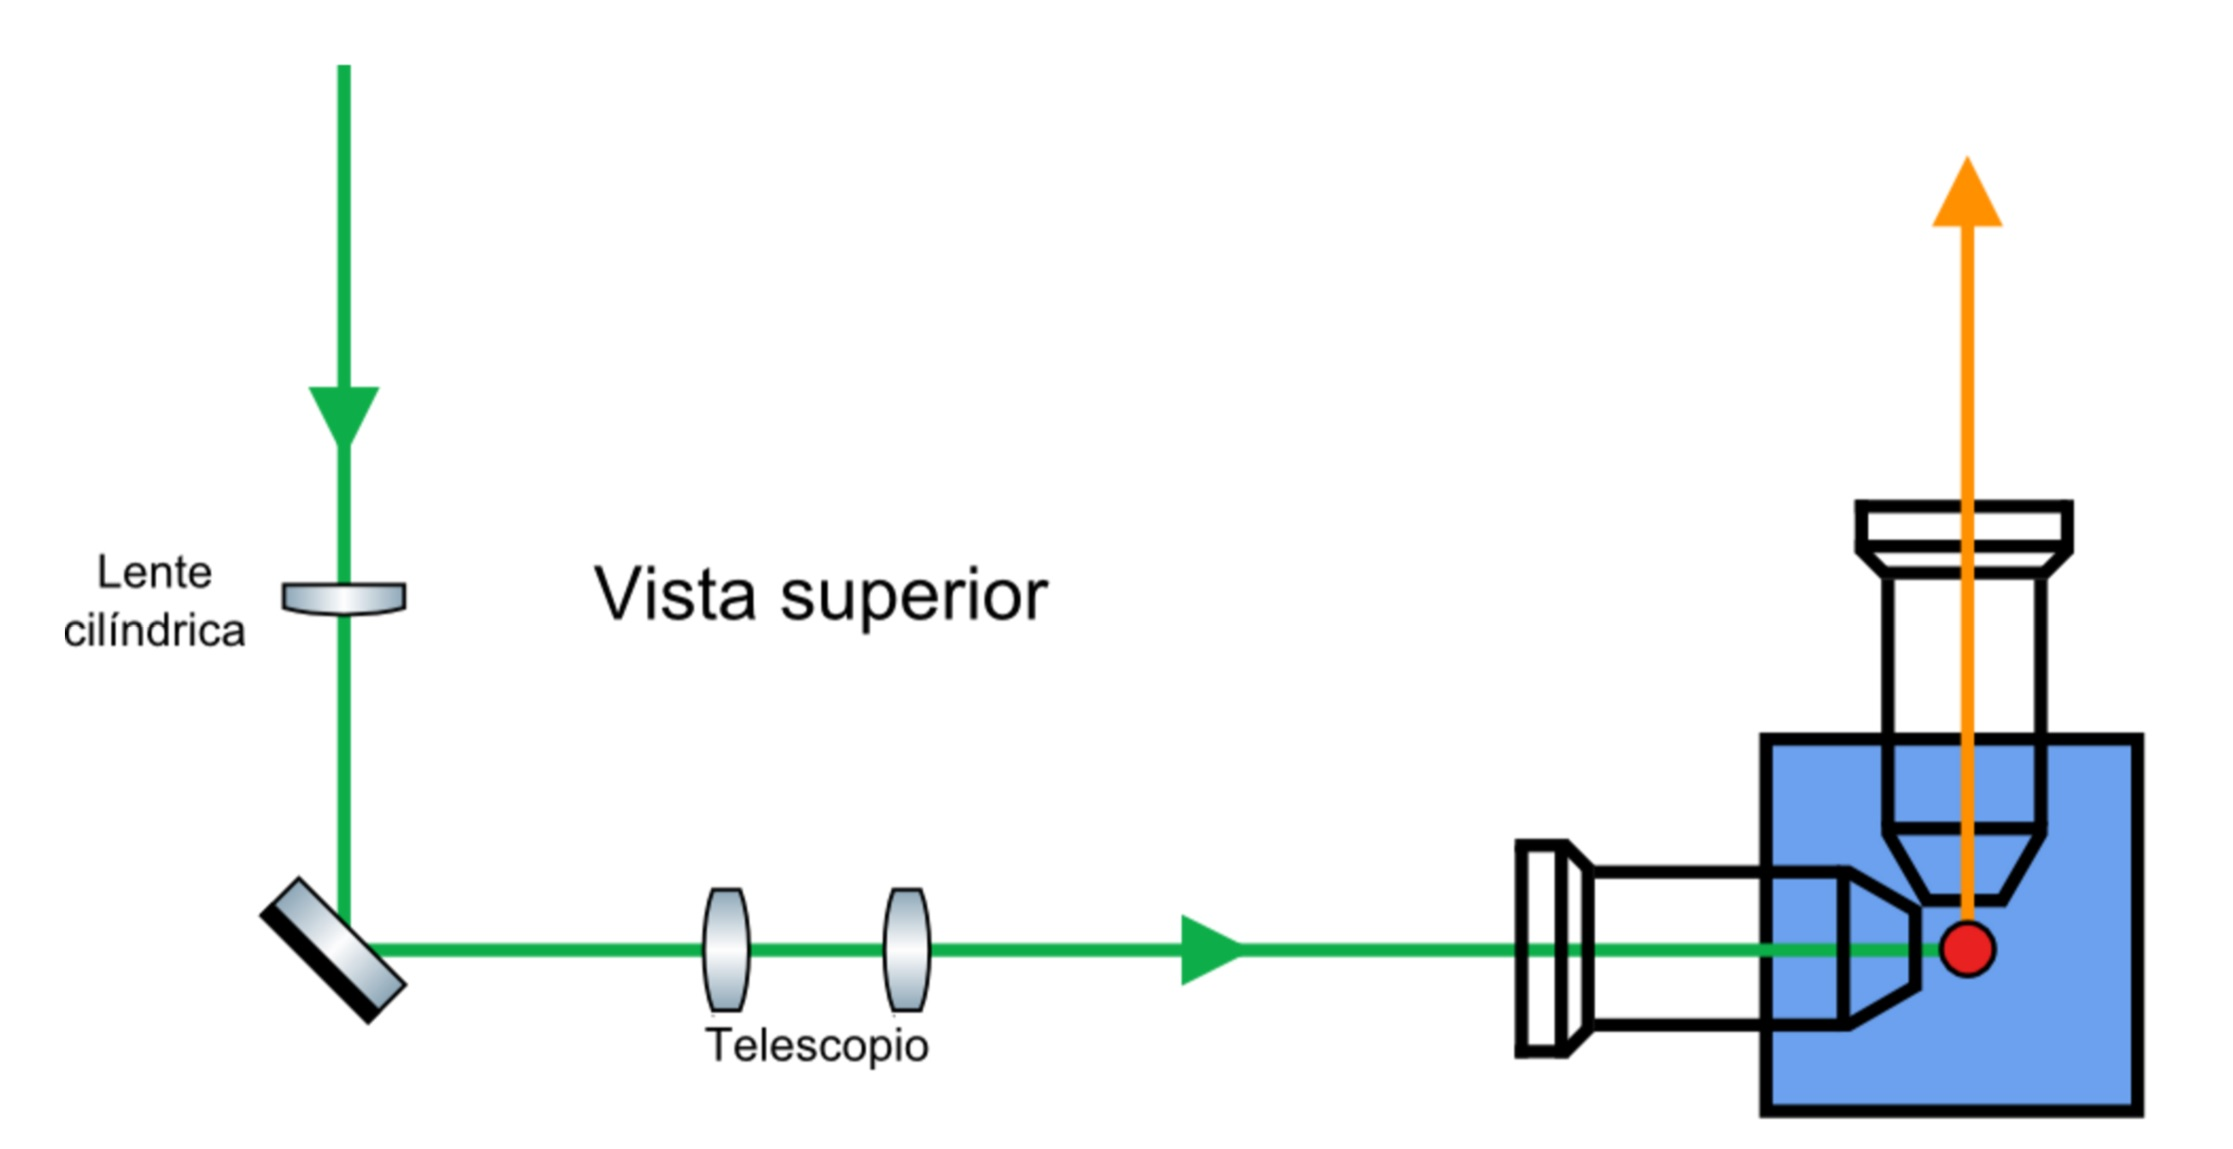
\includegraphics[width=0.6\textwidth]{fig/spim_lec}
    \caption{Esquema del microscopio SPIM del LEC, adaptado del trabajo de Huisken et al \cite{huisken2004}}
    \label{fig:spim_lec}
\end{figure}
En esta técnica se genera una hoja de luz (o \textit{lightsheet}) muy fina utilizando una lente cilíndrica. Iluminando a una muestra fluorescente con este \textit{lightsheet} y realizando una detección a 90$^{\circ}$, se logra excitar y observar a los fluoróforos de un único plano por vez. Barriendo la muestra en la dirección perpendicular del \textit{lightsheet} se colectan sucesivos planos que luego se combinan para hacer una reconstrucción tridimensional. Esto disminuye significativamente los niveles de photobleaching, es decir el blanqueado de los fluorforos, y fototoxicidad en comparación con técnicas como la microscopía confocal, en las que es necesario iluminar a la muestra completa para obtener cada plano. 

El microscopio construido en el laboratorio permite excitar fluoróforos en tres longitudes de onda (473$\,$nm, 532$\,$nm y 633$\,$nm) acopladas a una fibra óptica. Esto permite cambiar fácilmente la longitud de onda de excitación sin tener que realinear todo el sistema. A partir del análisis efectuado previamente, se concluyó que la resolución lateral del dispositivo está entre 677 y 691 nm y la resolución axial es de 5.21$\,\mu$m, con un \textit{lightsheet} de alrededor de 10$\,\mu$m de espesor. Esta resolución está en el orden de la utilizada en la referencia\cite{huisken2004} para realizar reconstrucciones tridimensionales con resolución celular del desarrollo de diversos organismos in vivo.

Uno de los objetivos del SPIM del laboratorio es poder medir la anisotropía de polarización de muestras biológicas. Esta medición consiste en iluminar las muestras con luz polarizada linealmente (en la eje mayor del lightsheet), y observar el cambio de polarización de la fluorecencia. Este proceso se encuentra esquematizado en la figura \ref{fig:fotoseleccion}, donde se produce un proceso de fotoselección de fluoroforos y posterior emisión de fluorecencia con cambios en la polarización.

\begin{figure}[H]
    \centering
    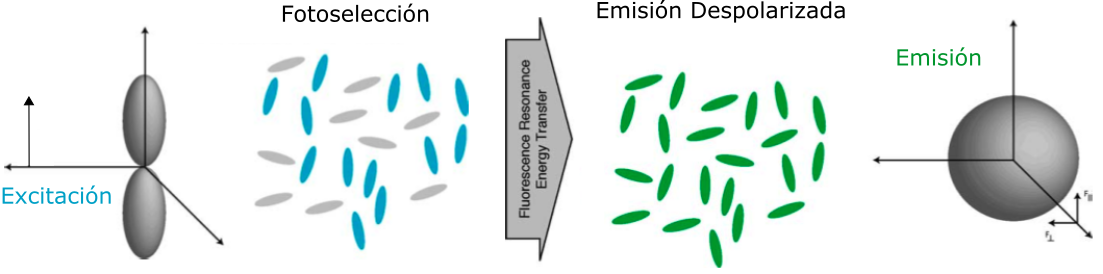
\includegraphics[width=0.8\textwidth]{fig/fotoseleccion}
    \caption{Esquema del proceso de fotoselección de flouroforos, para la posterior medición de la anisotropía}
    \label{fig:fotoseleccion}
\end{figure}

Esta magnitud permite medir procesos que cambian la estructura de los fluroforos, lo que representa un indicador para procesos biológicos de importancia para el laboratorio. De esta forma se busca poder adaptar el microscopio para poder hacer uso de estos sensores en las muestras; esto conlleva necesitar saber la polarización del haz a la salida de la fibra, para lo que también se necesita saber la polarización del haz a la entrada de dicha. La necesidad de medir la polarización se resuelve construyendo un instrumental para poder medirla, denomina de forma general como \emph{polarimetro}.

A la hora de optimizar el tamaño del \textit{lightsheet}, y por lo tanto la resolución del microscopio, es determinante la capacidad para caracterizar el perfil del haz en cada etapa.

Para efectuar esta caracterización en todo el experimento, es necesario armar paso a paso la experiencia, analizando la luz a la salida de cada etapa y adaptándola para el ingreso a la posterior sección. Además, este proceso es de naturaleza iterativa, es decir que debe repetirse más de una vez hasta alcanzar el objetivo buscado.

Si se necesita predecir el tamaño y la divergencia del haz a la salida de un elemento óptico, es necesario conocer el haz a la entrada y la relación entre el tamaño y la divergencia de entrada y salida. Para describir esta relación, tenemos una herramienta matemática llamada matrices ABCD\cite{svelto}.

Sean dos planos perpendiculares al eje óptico, uno de entrada y otro de salida. El haz cruza el plano de entrada a una distancia $x_1$ con un ángulo $\theta_1$ respecto a la normal del plano, y lo mismo para el plano de salida con $x_2$ y $\theta_2$. La relación entre las variables se pueden escribir como una transformación matricial de la forma
\begin{equation}
{x_2 \choose \theta_2} = \begin{pmatrix} A & B \\ C & D \end{pmatrix}{x_1 \choose \theta_1} = \boldsymbol{S}  {x_1 \choose \theta_1} ,
\end{equation}

donde los números $A$,$B$,$C$, $D$ dependen solamente del objeto óptico entre el plano de entrada y salida. 

Por ejemplo, la matriz
\begin{equation}
\boldsymbol{S} = \begin{pmatrix} 1 & d \\ 0 & 1 \end{pmatrix}
\end{equation}
representa un espacio vacío de distancia $d$ entre los planos con una distancia, ya que

\[ {x_2 \choose \theta_2} = \begin{pmatrix} 1 & d \\ 0 & 1 \end{pmatrix}{x_1 \choose \theta_1} = {x_1 + d \theta_1 \choose \theta_1} \]
donde para pequeños ángulos, donde $\sen(\theta) \approx \theta$, da el resultado esperado.

Otro ejemplo, más interesante, es la representación de una lente delgada con distancia focal $f$.
\begin{equation}
\boldsymbol{S} = \begin{pmatrix} 1 & 0 \\ -\frac{1}{f} & 1 \end{pmatrix}
\end{equation}

donde en el plano de salida tenemos que
\[  {x_2 \choose \theta_2} = \begin{pmatrix} 1 & 0 \\ -\frac{1}{f} & 1 \end{pmatrix}{x_1 \choose \theta_1} = {x_1 \choose -\frac{x_1}{f} + \theta_1}\]
es decir, achica el ángulo de salida del haz dependiendo de la distancia focal y el tamaño del haz, hecho que describe correctamente el funcionamiento de una lente delgada.

Cualquier sistema óptico puede ser descripto como un matriz ABCD, que constituye un método sistemático para el trazado de rayos.

Este método puede ser fácilmente aplicado para un haz gaussiano en propagación libre. Un haz gaussiano corresponde a un haz tal que plano perpendicular a la dirección de propagación tiene una intensidad gaussiana o una campana o función de Gauss, como se ve en la figura \ref{fig:gaussian_beam_profile}

\begin{figure}[H]
\centering
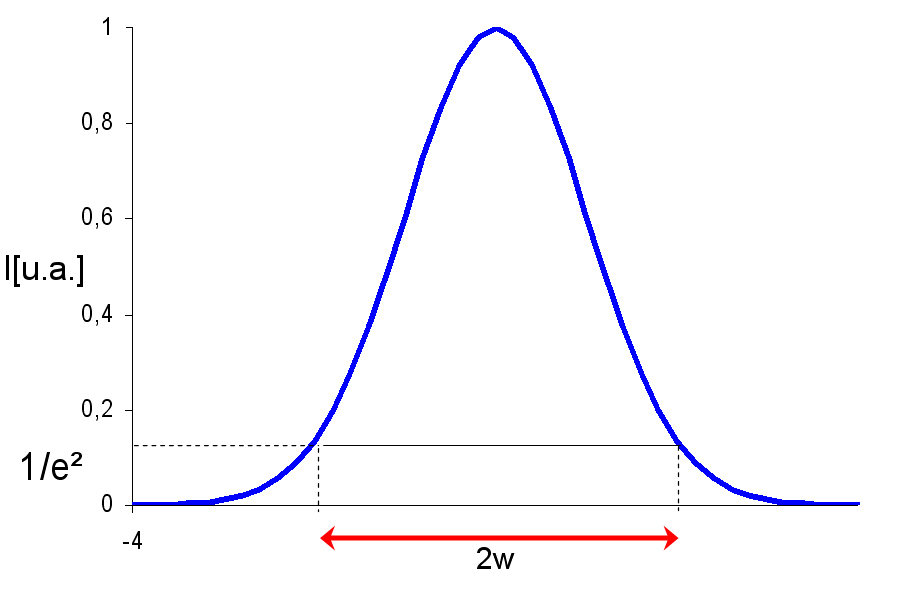
\includegraphics[width=0.35\textwidth]{fig/gaussian_beam_profile}
\caption{Perfil de intensidad de un haz gaussiano, con ancho o tamaño medio del haz parametrizado por w}
\label{fig:gaussian_beam_profile}
\end{figure}

Para estos haces se puede deducir el parámetro complejo del haz $q$ en la siguiente expresión \cite{svelto} 

\begin{equation}
    \frac{1}{q} = \frac{1}{R} - i \frac{\lambda}{\pi w^2}
    \label{eq:perfilacion/beam_parameter}
\end{equation}
donde $R$ es el radio de curvatura del haz, $lambda$ la longitud de onda y $w$ el ancho del haz. Con este parámetro y las matrices ABCD para la propagación libre ($A=D=1$, $B=z$ y $R\to\infty$, ya que no se curva el haz), se deduce que el ancho de un haz gaussiano $w$ en función del avance del haz $z$ se puede expresar como

\begin{equation}
    w(z) = w_0 \sqrt{1 + \left(\frac{\lambda z}{\pi w_0^2}\right)^2}
    \label{eq:perfilacion/gauss_divergence}
\end{equation}

donde $\lambda$ es la longitud de onda del haz y $w_0$ es la cintura del haz mínima, dada en el \emph{plano focal}. 

Este expresión se puede ver esquematizada en la figura \ref{fig:gaussian_beam_divergence}, que corresponde a un corte transversal a la propagación del haz, donde se puede apreciar la presencia del plano focal y como el haz converge y diverge de este plano

\begin{figure}[H]
\centering
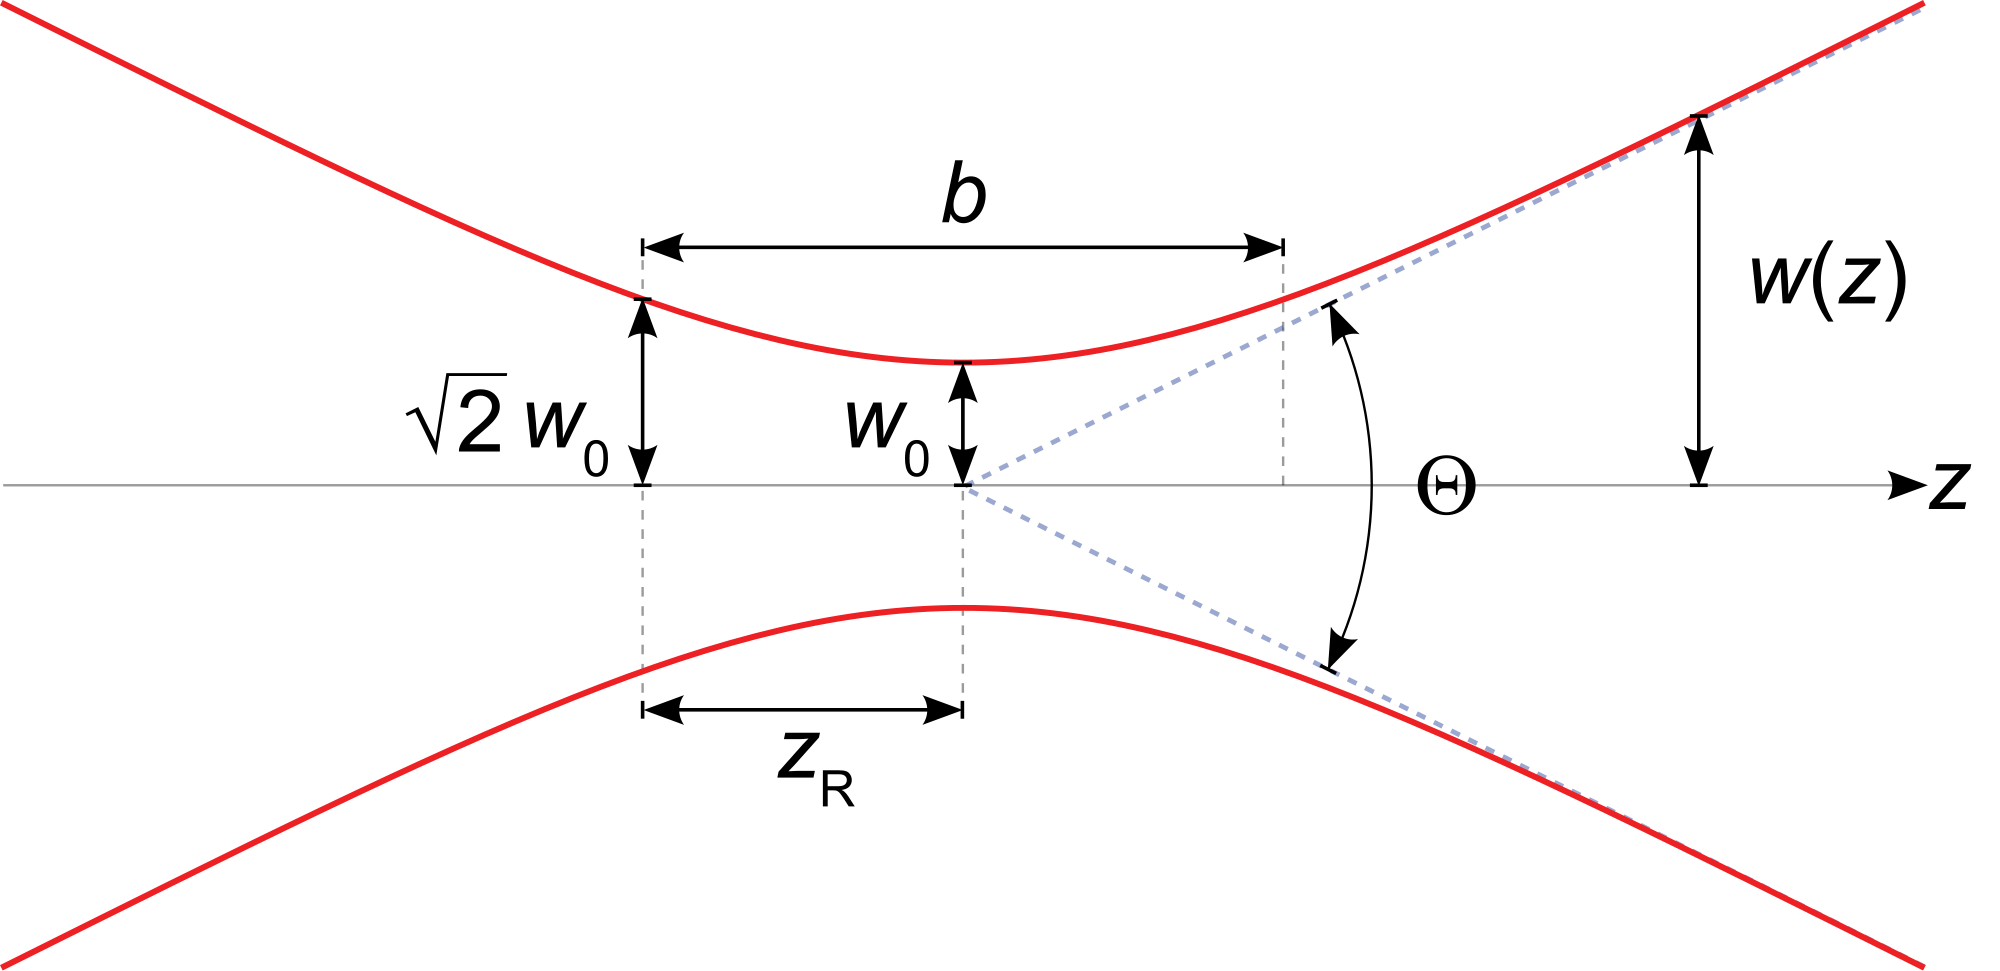
\includegraphics[width=0.35\textwidth]{fig/gaussian_beam_divergence}
\caption{Divergencia de un haz gaussiano, en este caso w$_0$ es el ancho medio mínimo del haz, en el plano focal}
\label{fig:gaussian_beam_divergence}
\end{figure}

De esta forma, el uso de matrices ABCD, especialmente para el caso guassiano, permite deducir todos los parámetros de haz y permite hacer predicciones teóricas sobre los distintos elementos ópticos utilizados en las experiencias en el laboratorio.

Para poder medir el perfil espacial y eventualmente la divergencia es necesario utilizar un perfilador de haz. Mientras tanto, para determinar la polarización de la fuente de luz se debe construir un polarimetro.

\subsection{Perfilador}

El método más usual para perfilar un haz consiste en ir obturando dicho haz y medir la potencia o intensidad del haz no obturado. El perfilador más sencillo que utiliza este concepto se puede observar en la figura \ref{fig:perfilador_basico}, que consiste en una hoja filosa (para aportar imperfecciones a la obturación) y un sensor de potencia o un sensor integrador de intensidad lumínica (como ser un fotodiodo). 

\begin{figure}[H]
\centering
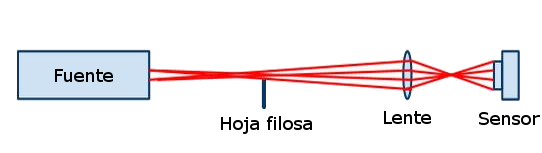
\includegraphics[width=0.35\textwidth]{fig/perfilador/esquema_basico}
\caption{Esquema de un perfilador manual}
\label{fig:perfilador/esquema_basico}
\end{figure}

Como la intensidad del haz que se mide en el fotodiodo o el sensor de potencia corresponde a la integral del haz, para un haz gaussiano vamos a observar una función error, que tiene la forma que se ve en la figura \ref{fig:err_function}

\begin{figure}[H]
\centering
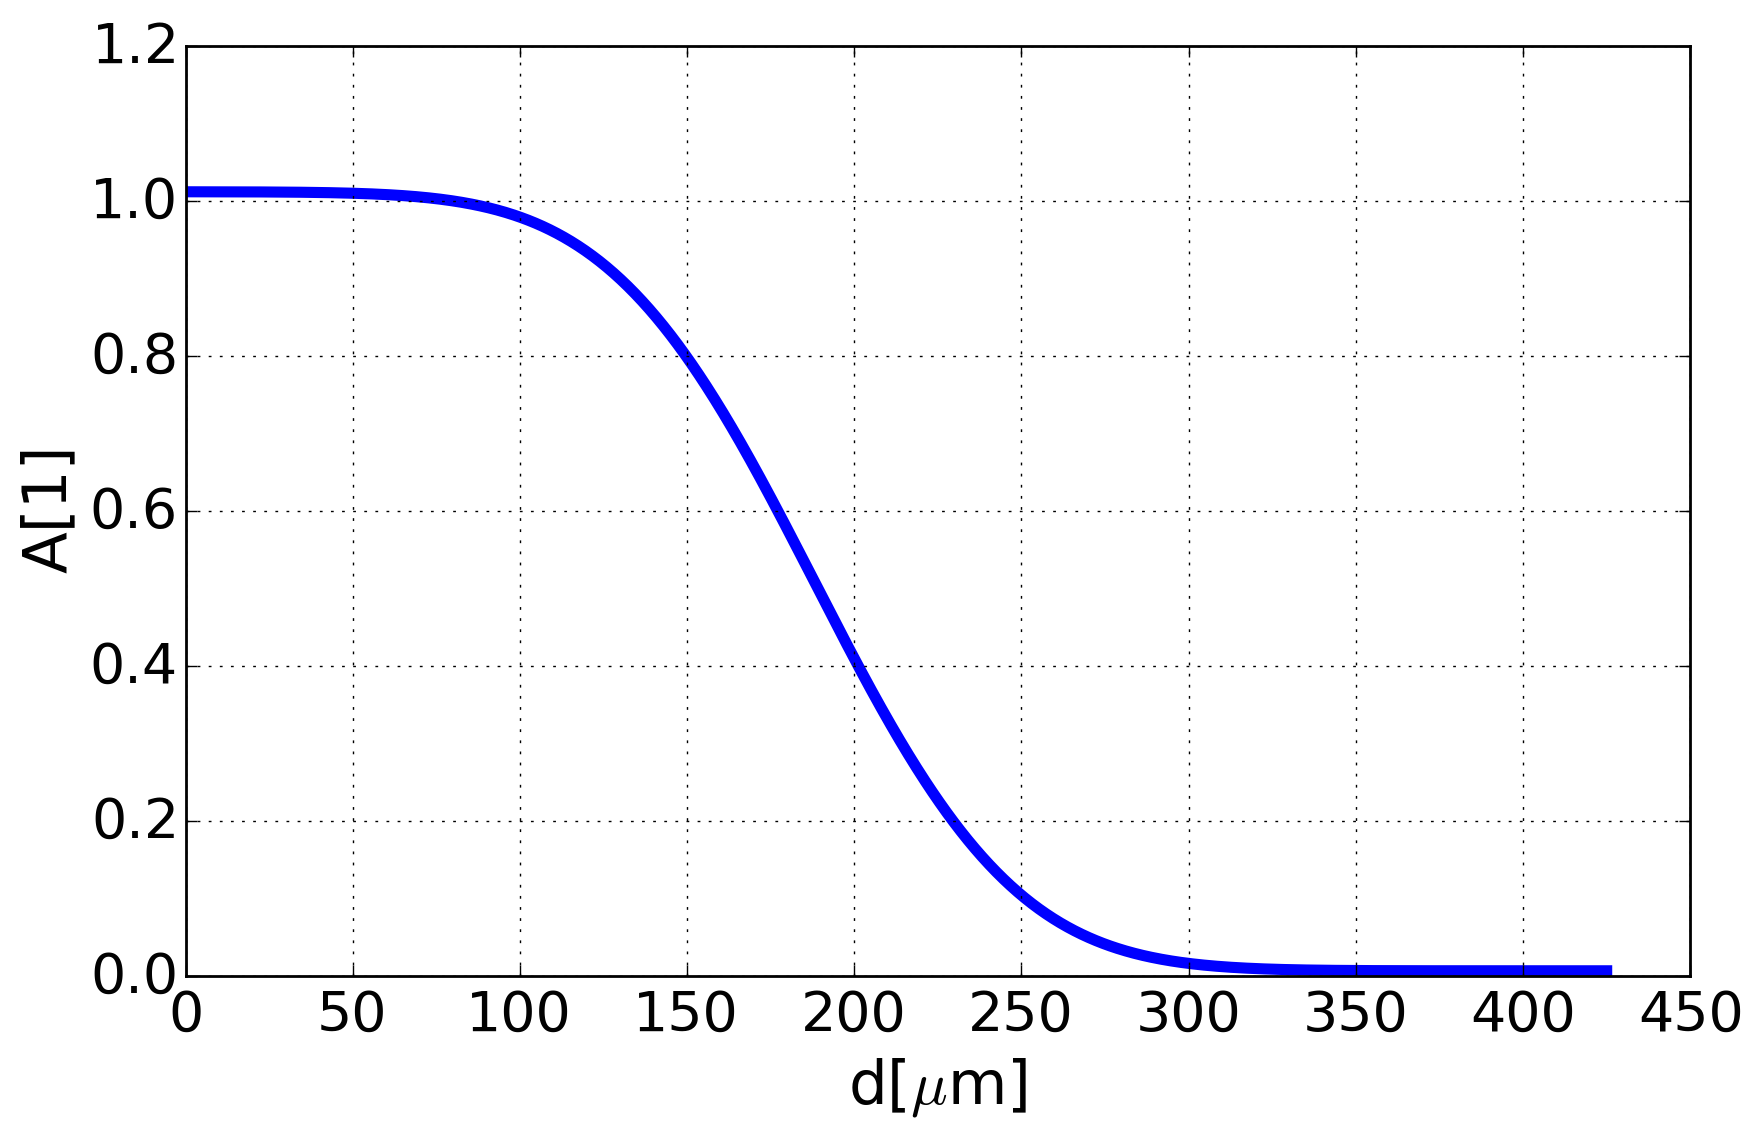
\includegraphics[width=0.4\textwidth]{fig/perfilador/err_function}
\caption{Simulación de la intensidad adquirida por un perfilador integrador en caso de un perfil gaussiano. Es un gráfico de la función error}
\label{fig:perfilador/err_function}
\end{figure}

El perfilador de Thorlabs \cite{thorlabs_profiler}, un referente comercial, consiste en un tambor giratorio con ranuras; el haz es obturado por la rendija, que define el ancho del perfil medido, la precisión la obturación y finalmente la dirección de la perfilación del haz. Después un sensor CMOS obtiene la intensidad del haz a la salida de la ranura, con su distribución espacial. 

Este perfilador es muy simple de operar, ya que no es necesario calcular ninguna derivada para observar el perfil, pero necesita un sensor CMOS con suficiente sensibilidad espacial y rango dinámico para las aplicaciones del instrumento. Esto conlleva a tener un instrumental caro solamente por el sensor, y además el equipo de Thorlabs tiene dimensiones prohibitivas para ser embebido en los setups utilizados en el laboratorio.

Mientras, el perfilador que se propone construir y caracterizar en este trabajo consiste en un tambor con rendijas (u otra estructura mecánica) que al girar obtura el haz y este es recolectado por un fotodiodo. Las rendijas o el mecanismo de obturación deben ser tal de poder obturar el haz en su totalidad y probablemente será necesario una lente para adaptar el perfilador a haces de diversos tamaños.

Otro objetivo del perfilador es lograr adquirir el perfil en tiempo real, para permitir acelerar el proceso de calibración y alineación de los setups del laboratorio. Para lograr visualizar cada medición de forma suave, la velocidad del motor y la adquisición de datos debe permitir medir perfiles y presentar en pantalla unas 24 veces por segundo, que es el límite de percepción humana donde el movimiento empieza a ser fluido.

Sin embargo, se debe considerar una medición manual del perfilador requiere entre 5 y 10 minutos, además del tiempo de colocación del instrumental, por lo que lograr medir entre 5 y 10 veces por segundo representaría una mejora subtancial al proceso de alineación y calibración.

Esta velocidad de refresco va a determinar la velocidad del tambor y la velocidad de la adquisición y acondicionamiento de los datos.

\subsection{Polarímetro}

Mientras tanto, un polarímetro es un instrumento capaz medir las propiedades de la polarización de una fuente óptica.

El modelo conceptual a utilizar se puede observar en la figura \ref{fig:polarimetro/esquema}. Este consiste en una lámina polarizadora lineal que puede rotar en un coaxial o perpendicular al plano de polarización, y al hacer este movimiento va cambiando el plano de polarización. En cada nuevo plano se transforma la luz transferida en señal eléctrica con un sensor integrador como un sensor de potencia o un fotodiodio. 

\begin{figure}[H]
    \centering
    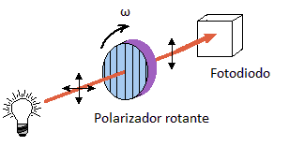
\includegraphics[width=0.45\textwidth]{fig/polarimetro/esquema}
    \caption{Esquema conceptual del polarímetro, donde se observa la fuente de luz, con alguna polarización a determinar, la lámina rotante polarizadora y el sensor de luz integrador, en este caso un fotodiodo}
    \label{fig:polarimetro/esquema}
\end{figure}

Si uno mide la intensidad de un haz linealmente polarizado que atravieza una lámina polarizadora lineal se observará la ley de Malus \cite{goldstein_collete}, que tiene la expresión
\begin{equation}
    I(\theta) = I_0 \cos^2(\theta)
    \label{eq:malus}
\end{equation}
donde el ángulo $\theta$ corresponde al ángulo de proyección entre el campo eléctrico incidente y el eje de la lámina. De esta forma esta expresión expresa la intensidad observada en la figura \ref{fig:polarizacion/malus}

\begin{figure}[H]
    \centering
    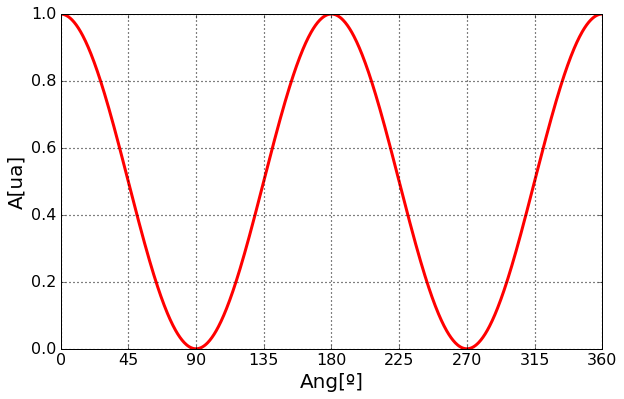
\includegraphics[width=0.38\textwidth]{fig/polarimetro/malus}
    \caption{Intensidad en función de ángulo de rotación de lámina polarizadora según la ley de Malus}
    \label{fig:polarizacion/malus}
\end{figure}

Sin embargo, si la fuente está elipticamente polarizada, uno no observará la ley de Malus si no una expresión del estilo \cite{goldstein_collett}
\begin{equation}
    I(\theta) = I_0 \cos^2(\theta) + I'_0
\end{equation}
donde la intensidad $I'_0$ agrega un offset debido a qué en hay intensidad de luz en el eje menor de la polarización. En el caso de ser circular directamente se observa una intensidad constante y si se observa polarización aleatoria no se podría hacer ningún ajuste a los datos o si el cambio de la polarización es muy rápido puede que se observe una intensidad constante.

Recordemos que el primer objetivo del polarizador es determinar el cambio de polarización que se produce al atravezar la fibra. El resultado óptimo es que a la salida de la fibra haya una polarización lineal, pero el único resultado limitante para futuras mediciones es una polarización aleatoria a la salida de la fibra. Cualquier tipo de polarización estable puede alterarse con láminas retardadoras. 

Para cuantificar la polarización a partir de la intensidad adquirida del fotodiodo se define un coeficiente de \emph{calidad de polarización lineal}, definido como
\begin{equation}
    \alpha = \frac{\max - \min}{\max + \min} = \begin{cases} 1 & \text{lineal} \\ 0 & \text{circular} \\ 0 < \alpha < 1 & \text{eliptica} \end{cases}
    \label{eq:polarizacion/alpha}
\end{equation}
que asigna un rango numérico a los tipos de polarización posible. Si la fuente tuviese una polarización aleatoria, entonces no se podría ajustar la ley de Malus o una constante correctamente.

Respecto a la velocidad de adquisición del instrumental, nuevamente se requiere adquirir en tiempo real, para poder observar la polarización mientras se altera láminas retardadoras y la alineación de algunos elementos ópticos. Dado que una medición manual tarda entre 5 a 10 minutos, con lograr entre 5 y 10 mediciones por minuto se acortaría considerablemente los tiempos de trabajo.

    %\section{Objetivos}
    \section{Desarrollo experimental}
        
El diseño de estos instrumentales está enmarcado en el proyecto SOMA\cite{soma}, de Sistemas de OptoMecánica Abierta, del LEC. Este proyecto tiene como objetivos crear herramientas e instrumentos optomecánicos capaces de ser repetibles con facilidad, y con todo los diseños, de las partes que los integran, libres a la comunidad. Libres en este contexto significa que pueden ser utilizados para repetir la implementación del perfilador o mejorarlos para toda la comunidad.

De esta forma, todos los diseños fueron efectuados con metodologías automatizadas, en particular los prototipos se hicieron con la impresora 3D del departamento, además la electrónica utilizada es libre, y el software de adquisición de datos está hecho en plataformas de desarrollo y librerías libres.

\subsection{Perfilador}

El diseño y la tecnología necesaria para el funcionamiento del perfilador empezó a dilucidarse en Laboratorio 6, y para final de Laboratorio 7 se reaplicó con éxito al polarimetro. Las partes mecánicas a diseñar y construir para el perfilador consistieron en el tambor, encargado de obturar el haz, el actuador o motor del tambor, que debe ser adquirido, y el soporte para el tambor y el motor. 

En la figura \ref{fig:perfilador/esquema_bloques} se muestra un diagrama en bloques del perfilador, para tener noción de los componentes que representan y que partes fueron creadas

\begin{figure}[H]
    \centering
    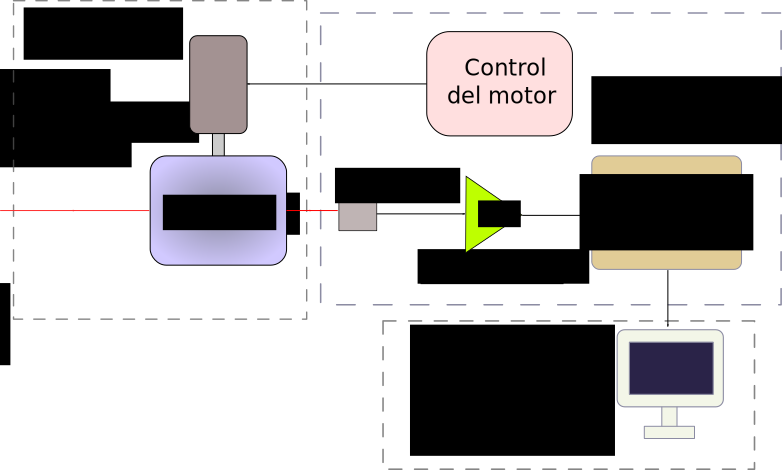
\includegraphics[width=0.6\textwidth]{fig/perfilador/esquema_bloques}
    \caption{Diagrama en bloques del perfilador construido}
    \label{fig:perfilador/esquema_bloques}
\end{figure}

El diseño de la electrónica y la adquisición de los datos se trata en un apartado aparte ya que tiene directa aplicación al polarimetro, además del perfilador.

\subsubsection{Tambor}
Como la velocidad de rotación del tambor, al menos la velocidad objetivo, es de 24 revoluciones por segundo, no se consideró, a priori, hacer un análisis del material a utilizar. Esto se justifica considerando que aún siendo 1440 revoluciones por minuto, es una velocidad bastante inferior a la velocidad de los  motores de alterna, que giran a 3000RPM, y las piezas de plástico impresas se saben que mantienen la estructura intacta a esas velocidades. De esta forma se construyó en plástico, con la impresora 3D, el tambor y se observó experimentalmente su funcionamiento.

El primer diseño, y único diseño salvo cambios de dimensiones, del tambor, consistió en un cilindro macizo de 15$\,$cm de diámetro, con un corte perpendicular al eje, hasta 5$\,$mm después de cruzar el eje, como se ve en la figura \ref{fig:perfilador/tambor}. Esto permite al girar el tambor ir cortando el haz, como se ve en la figura \ref{fig:perfilador/corte_tambor}, en este caso con un diámetro de hasta 10$\,$mm. 


\begin{figure}[H]
    \begin{subfigure}[b]{0.45\textwidth}
        \centering
        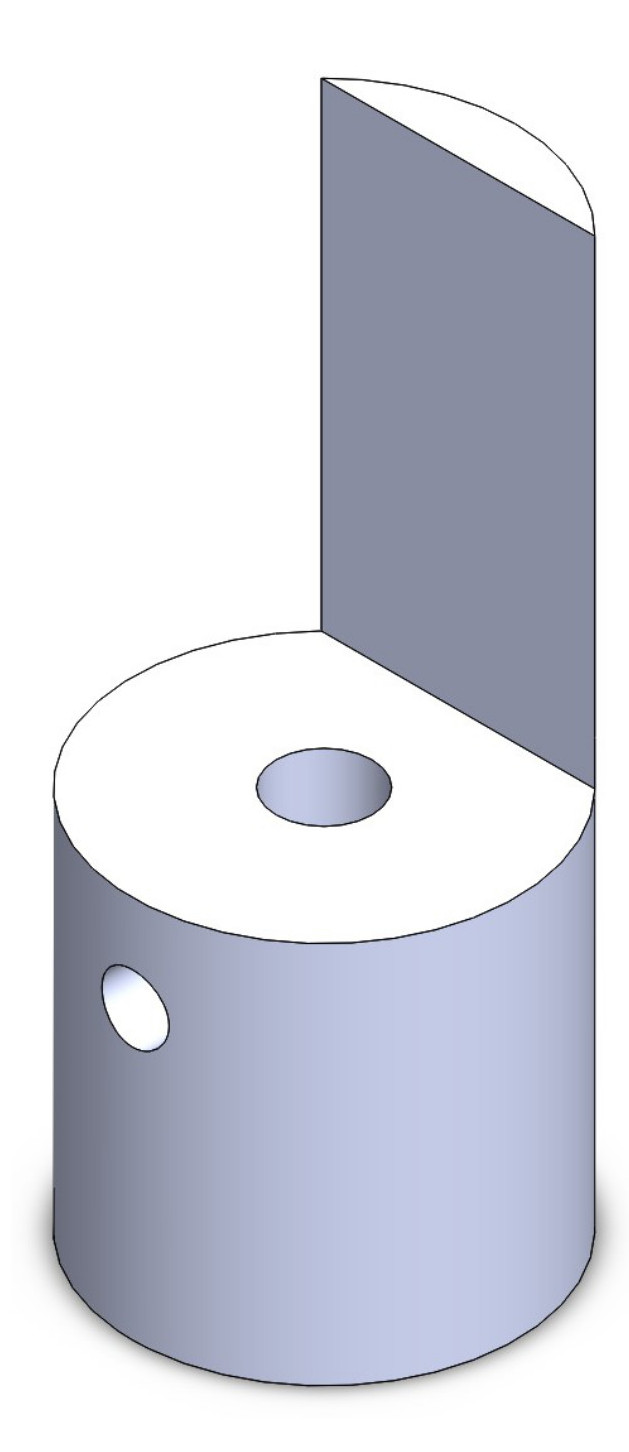
\includegraphics[width=0.5\textwidth]{fig/perfilador/tambor}
        \caption{}
        \label{fig:perfilador/tambor}
    \end{subfigure}
    \begin{subfigure}[b]{0.45\textwidth}
        \centering
        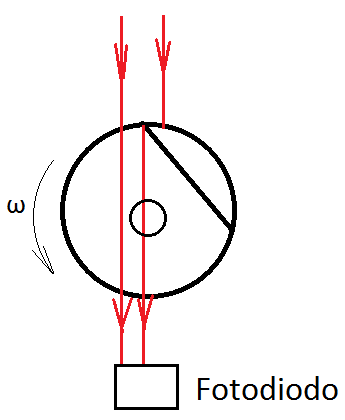
\includegraphics[width=0.6\textwidth]{fig/perfilador/corte_tambor}
        \caption{Esquema de la obturación}
        \label{fig:perfilador/corte_tambor}
    \end{subfigure}
    \caption{Tambor del perfilador}
\end{figure}

Este diseño permite que el tambor pueda entrar en compartimientos pequeños, y en particular se busca que el tambor entre en el interior de un sistema Cage Ø1'' de Thorlabs \cite{thorlabs_cage}; el sistema Cage representa uno de los entornos de trabajo más usuales del laboratorio, por lo que es necesario adaptar el perfilador a este.

La necesidad de usar una prolongación para obturar en vez de una ranura es producto de una decisión de diseño. Si el tambor con ranuras está entre el sensor y la fuente del haz, el sensor va a observar una obturación errónea, ya que el el haz va a ser obturado por la ranura de entrada del tambor y la ranura de salida, como se ve diagramado en la figura \ref{fig:perfilador/tambor_ranuras}. Debido a esto, es necesario obturar con la prolongación.

No solo eso, la prolongación permite obturar el haz hasta 4 veces por vuelta, dos veces dos planos diferentes del haz. Esto a su vez permitiría medir la divergencia, si es el haz diverge de forma apreciable en 20$\,$mm, el diámetro de cilindro, de de recorrido y también permite promediar dos obturaciones por plano en una vuelta. 

\begin{figure}[H]
\centering
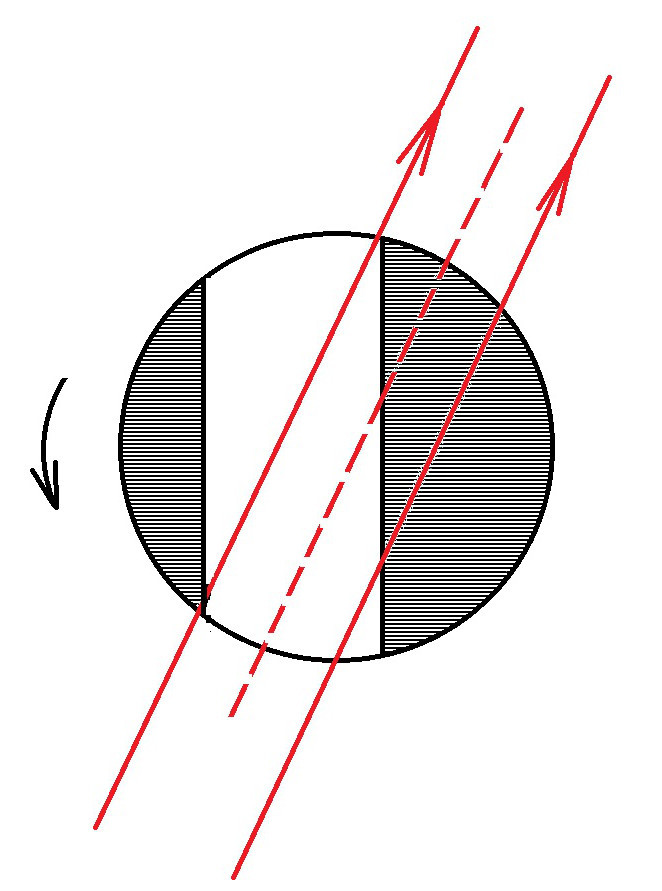
\includegraphics[width=0.25\textwidth]{fig/perfilador/tambor_ranuras}
\caption{Corte transversal de un tambor con ranuras, donde se observar la ranura obturando un haz.}
\label{fig:perfilador/tambor_ranuras}
\end{figure}

Sin embargo, debe considerarse que la prolongación puede traer problemas mecánicos al rotar muy rápido, como ser una precesión al rotar o movimientos erráticos de la prolongación, que pueden producir mediciones del perfil erróneas. Por eso es de vital importancia medir el perfil del haz, en ambos planos de obturación, con otro perfilador.

De esta forma se construyó este diseño del tambor en aluminio, que tiene como ventaja menos oscilaciones al rotar y además tiene un filo más definido, pero lo que obtura el haz de forma más precisa. Sin embargo, la diferencia en tiempo de fabricación del tambor no justifica la mejora mecánica y además se necesita hacerle un proceso de galvanizado para no reflejar el haz al ambiente.


\subsubsection{Motor}

La velocidad de tambor debe ser tal que permita al perfilador generar una presentación de las mediciones con cinemática suave, que se logra adquiriendo y presentando con un refresco de 24 veces por segundo. Esto implica que el motor debe girar como mínimo a 24RPS (revoluciones por segundo) o 1440RPM.

Con esa premisa, se probaron todos los tipos de motores de corriente continua del mercado. Los motores de corriente altera y trifásicos se descartaron ya que no existen modelos de pequeñas dimensiones y exigen muchas precauciones eléctricas para su uso en una mesa óptica.

Como solución se eligieron los motores paso a paso. Un motor paso a paso corresponde a un motor de continua con un estator dentado con dos o más fases, como se ve en la figura \ref{fig:stepper_inner}. Al activar y desactivar en una secuencia la corriente por las fases se logra mover el rotor solamente un diente del estator o, lo que se denomina, un paso. Respecto a otros motores de continua tiene la ventaja de bloquearse si se pierde el sincronismo entre el rotor y el campo inducido, por lo que mantienen la velocidad de forma constante. Aún así pueden saltearse pasos si el torque a efectuar es muy grande, y con ello traería un problema en la medición. 

\begin{figure}[H]
\centering
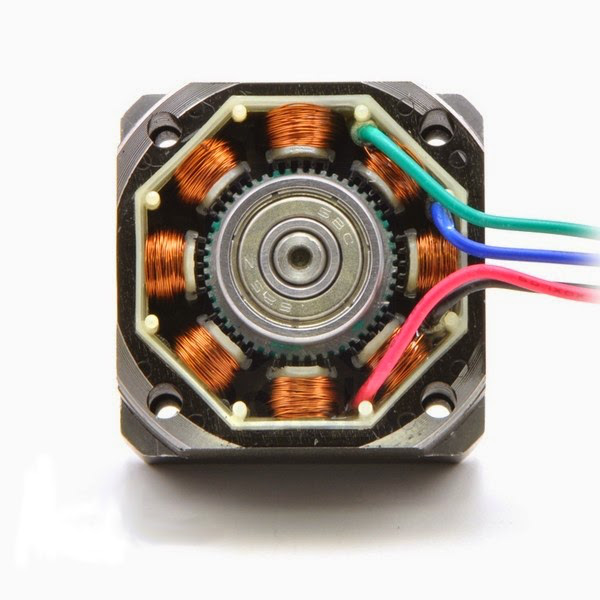
\includegraphics[width=0.3\textwidth]{fig/stepper_inner}
\caption{Motor paso a paso por dentro, donde se ve las diferentes fases y la rueda dentada}
\label{fig:stepper_inner}
\end{figure}

El motor paso a paso inicialmente adquirido corresponde al 42BYGHW609\cite{42BYGHW609}, con 200 pasos por vuelta y un torque de funcionamiento de 4$\,$kg$\,$cm. Este motor tiene la denominación NEMA 17, que determina el tamaño, 42,3$\times$42,3$\times$40$\,$mm, del motor y la ubicación de los agujeros de soporte. En la hoja de datos se observa que, en régimen de trabajo, se puede alcanzar una velocidad de 3000 pasos por segundo, es decir a 15RPS, con un torque de funcionamiento de 3kg$\,$cm; aún cuando esta información debe ser verificada experimentalmente, esto indica que el motor puede llegar a alcanzar las velocidades objetivo. 

El motor para alcanzar velocidades superiores a 10RPS necesita una aceleración constante, ya que debe cambiar el estado de movimiento de la inercia del eje y lo que tenga adosado en dicho. La electrónica de control, que es la misma que de adquisición, resuelve eso alterando la frecuencia de los pasos hasta llegar a la velocidad objetivo.

Después de efectuar pruebas y mediciones preliminarnes, en Laboratorio 6 principalmente, con el motor NEMA 17, se adquirió un motor NEMA 8, modelo 8H2A28402, con dimensiones 20$\times$20$\times$28$\,$mm y 200 pasos por vuelta, como el modelo anteriormente utilizado. Este motor se logró hacerlo girar a 30RPS, con un cambio de la electrónica de control involucrada, y a esa velocidad pudo mover el tambor de plástico así como el de metal. De esta forma el motor rota más rápdido que la velocidad necesaria originalmente, sobrepasando las expectativas. Este motor también requiere de una aceleración menor para alcanzar altas velocidades, pero al tener menor inercia se alcanzó con mayores aceleraciones la velocidad final. Esto conlleva a menores tiempos en arrancar a medir y además menores tiempos muertos.

\begin{figure}[H]
    \begin{subfigure}[b]{0.45\textwidth}
        \centering
        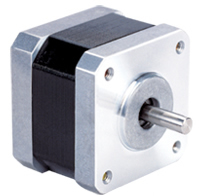
\includegraphics[width=0.7\textwidth]{fig/motor/nema17}
        \caption{Motor NEMA 17}
    \end{subfigure}
    \begin{subfigure}[b]{0.45\textwidth}
    \centering
        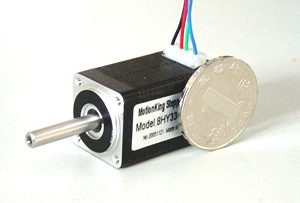
\includegraphics[width=0.7\textwidth]{fig/motor/nema8}
        \caption{Motor NEMA 8}
    \end{subfigure}
    \caption{Imagenes de los motores paso a paso utilizados. El eje de ambos motores mide 24$\,$mm, lo que dislumbra la diferencia en tamaño.}
\end{figure}

Este motor, al tener la mitad de tamaño en cada dimensión, permite diseñar un soporte que sea más fácil de integrar y medir en setups con limitaciones más importantes de espacio, además de achicar gastos en producción del soporte.

\subsubsection{Soporte}

El soporte del motor, el cuerpo principal del perfilador, fue diseñado considerando los setups usuales del laboratorio y la premisa básica de no desarmar ninguna estructura del experimento. 

El primer prototipo, que se ve en la figura \ref{fig:soporte_v1}, usa el motor NEMA 17 y entra en el sistema óptico paralelo al plano óptico, es decir por un costado del setup. Este soporte a su vez tiene un agujero donde descansa el sensor, a 50$\,$mm de la mesa óptica (que representa la altura usual del laboratorio), y puede pegarse una lente con una distancia focal como máxima de 10$\,$mm para adaptarse para haces más grandes. En el costado tiene agujeros para ajustar el motor. Con el motor atornillado el prototipo tiende a caerse, por lo que es necesario ajustarlo a la mesa óptica. Este soporte no es autoportante.

\begin{figure}[H]
\centering
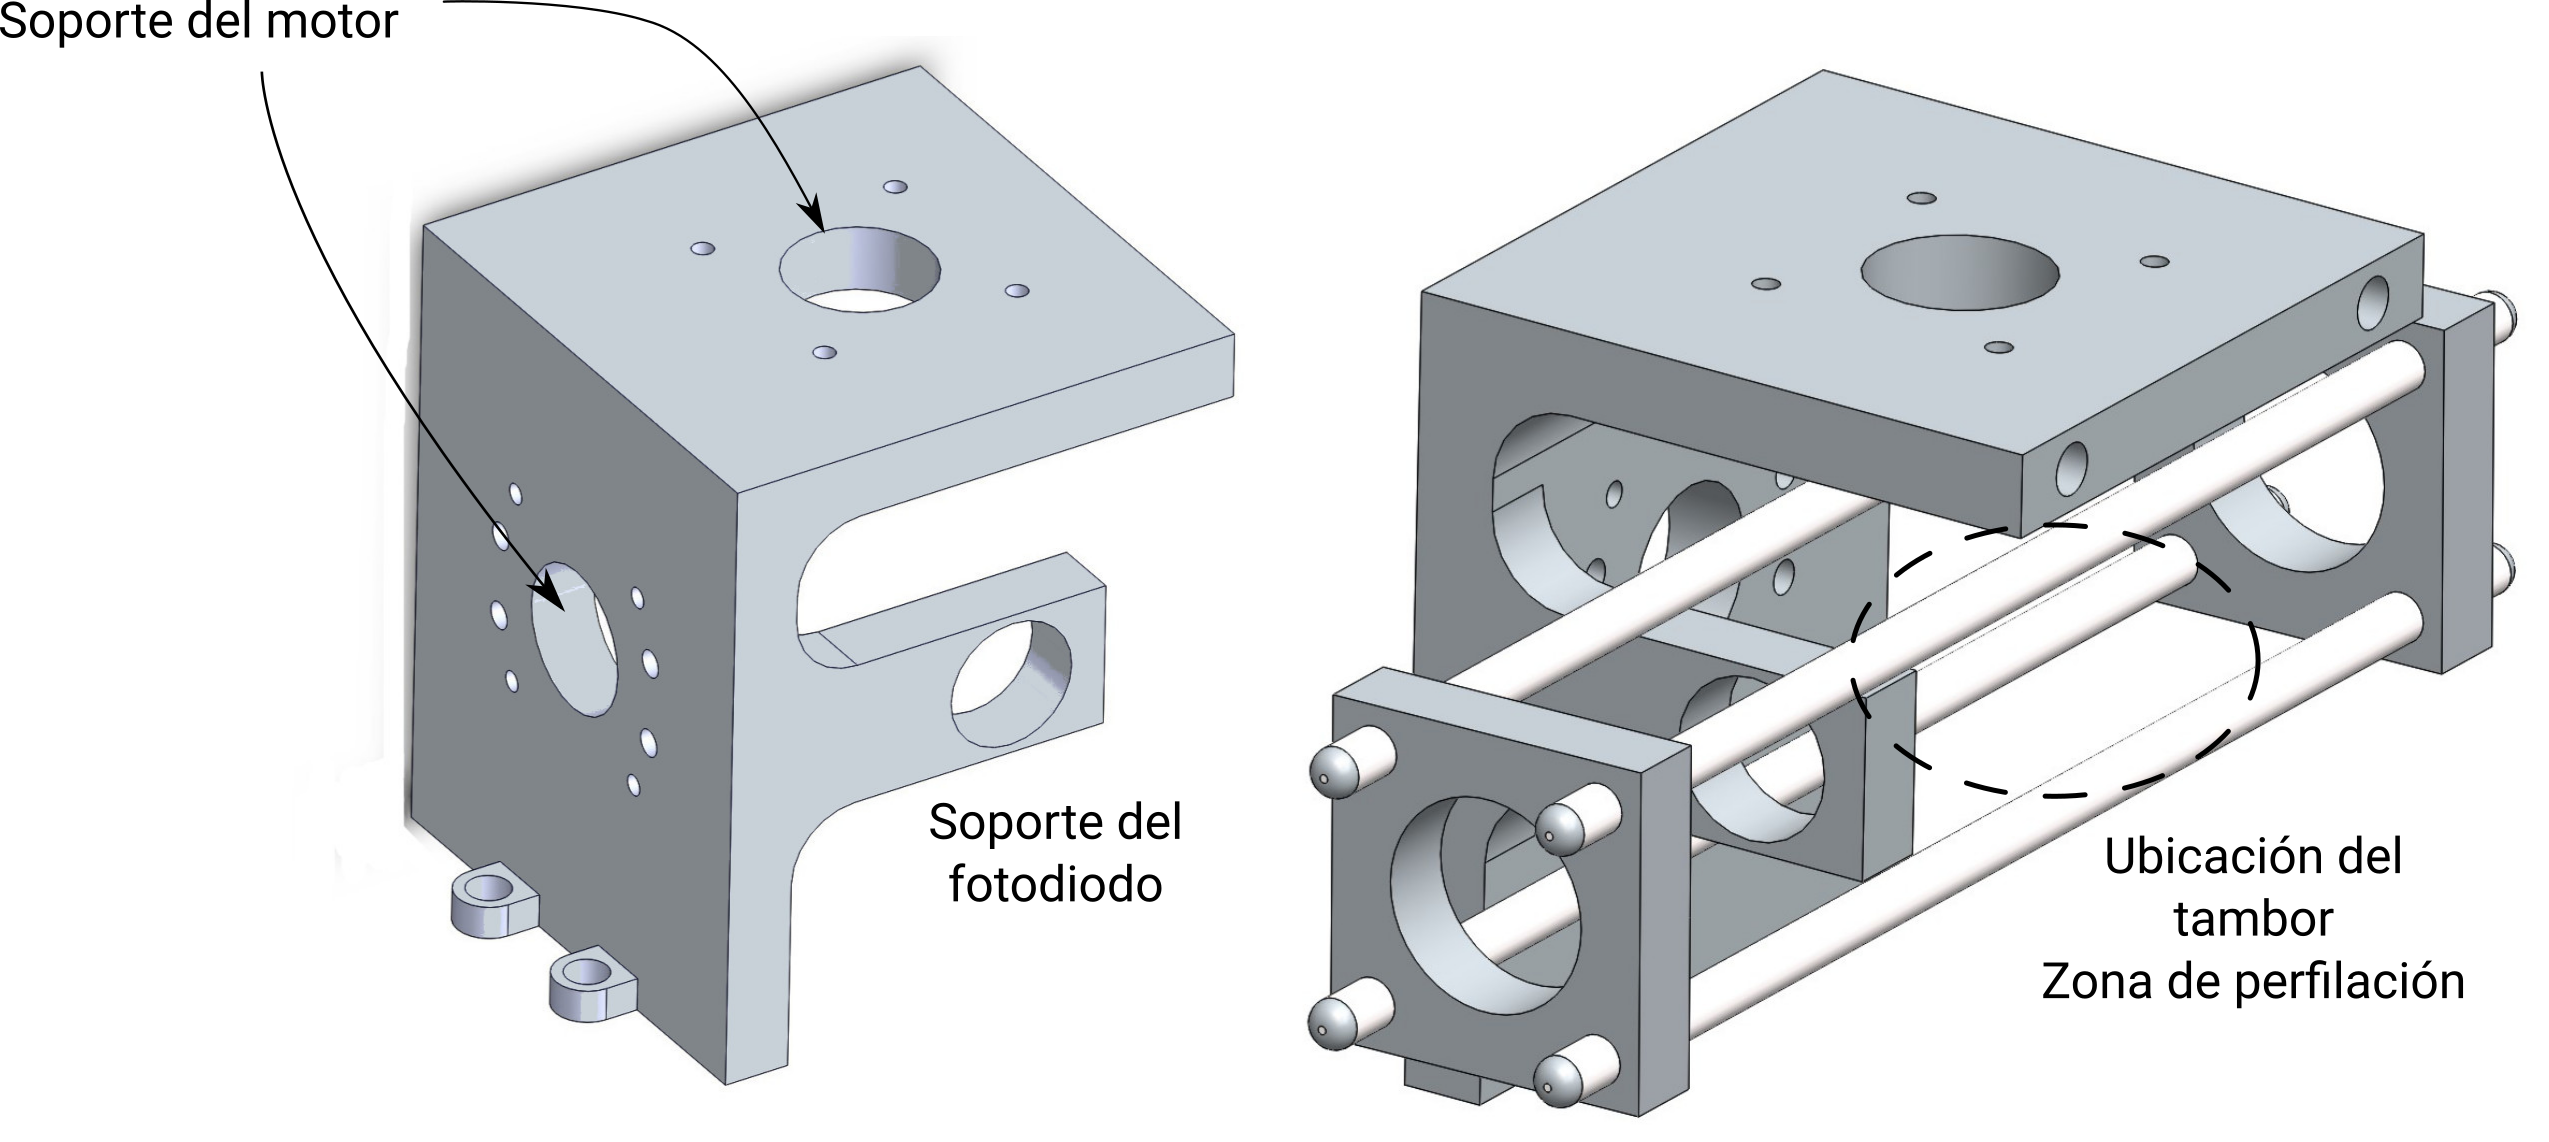
\includegraphics[width=0.65\textwidth]{fig/perfilador/soporte_v1}
\caption{Vista 3D del primer prototipo del soporte, junto con en ensamble en un posible Cage.}
\label{fig:soporte_v1}
\end{figure}

Los agujeros de más en el plano izquierdo permiten atornillarlo al soporte de poste de Thorlabs, pero este diseño en esa situación solo permite perfilar en sólo eje.

El segundo prototipo, también con el motor NEMA 17, consiste en un un diseño autoportante como se ve en la figura \ref{fig:soporte}. Este soporte entra al plano óptico perpendicular a este, es decir por arriba de la mesa óptica.

\begin{figure}[H]
\centering
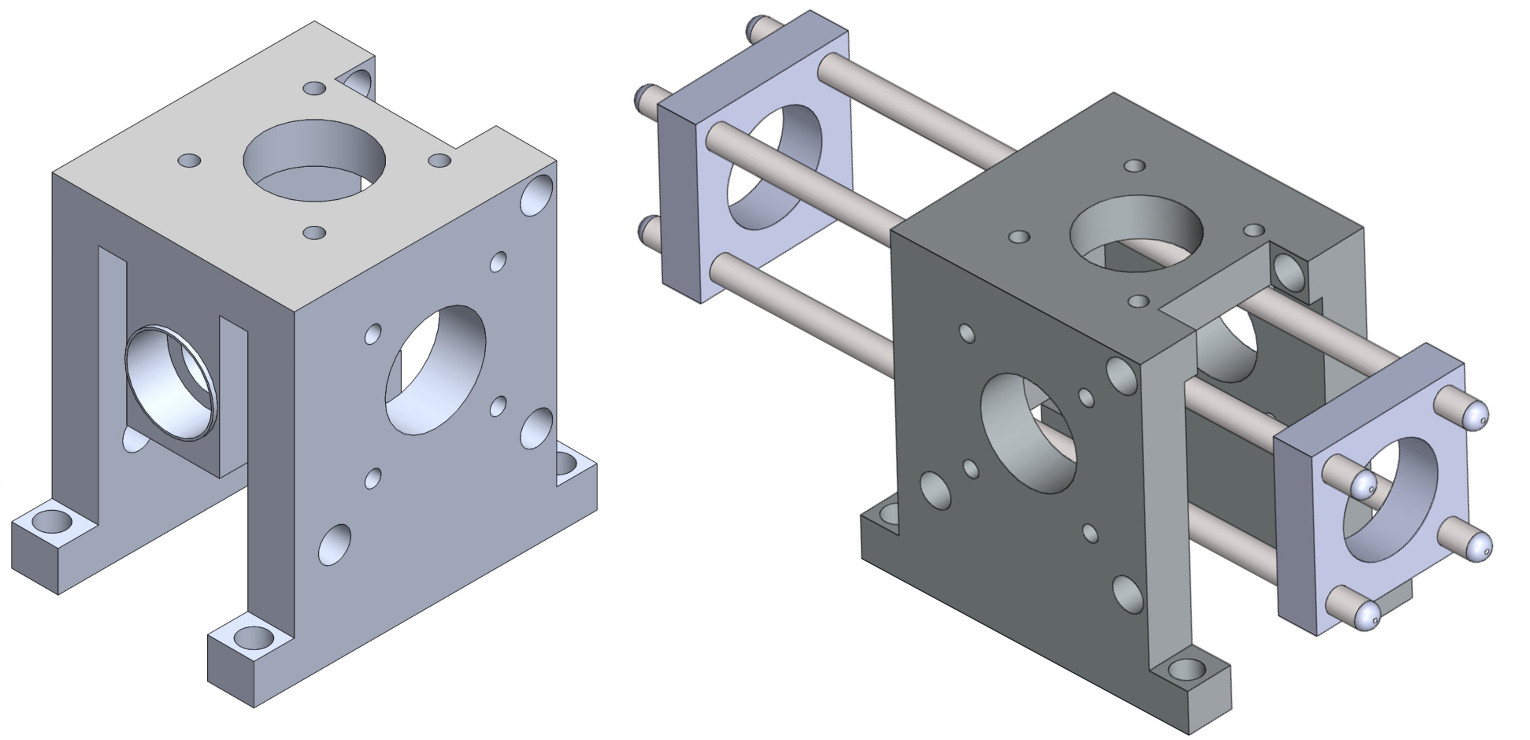
\includegraphics[width=0.65\textwidth]{fig/perfilador/soporte_v2}
\caption{Vistas tridimensionales del soporte, con el ensamble en un posible Cage.}
\label{fig:perfilador/soporte_v2}
\end{figure}

Este diseño tiene la ventaja soportar el motor sin la necesidad de ser atornillado y de poder medir en ambos ejes al estar adosado al soporte para postes de Thorlabs.

Ningún agujero tiene rosca, y además se los hicieron pasantes para los tornillos a utilizar; esto se debe a los límites impuestos por la impresora 3D utilizada. La mayoría del los agujeros tienen hasta 1$\,$mm más de diámetro para resultar pasantes en la impresión.

Habiendo hecho mediciones con ambos soportes, se llegó a la conclusión que el motor necesita estar encastrado para no generar problemas mecánicos en la medición. De esta forma el tercer prototipo del soporte, visto en la figura \ref{fig:perfilador/soporte_v3}, permite una muy rápida colocación en la mesa óptica. El sensor nuevamente descanza a 50$\,$mm de la mesa, y el largo de la prolongación permite medir correctamente cerca de un riel o en un Cage.

\begin{figure}[H]
\centering
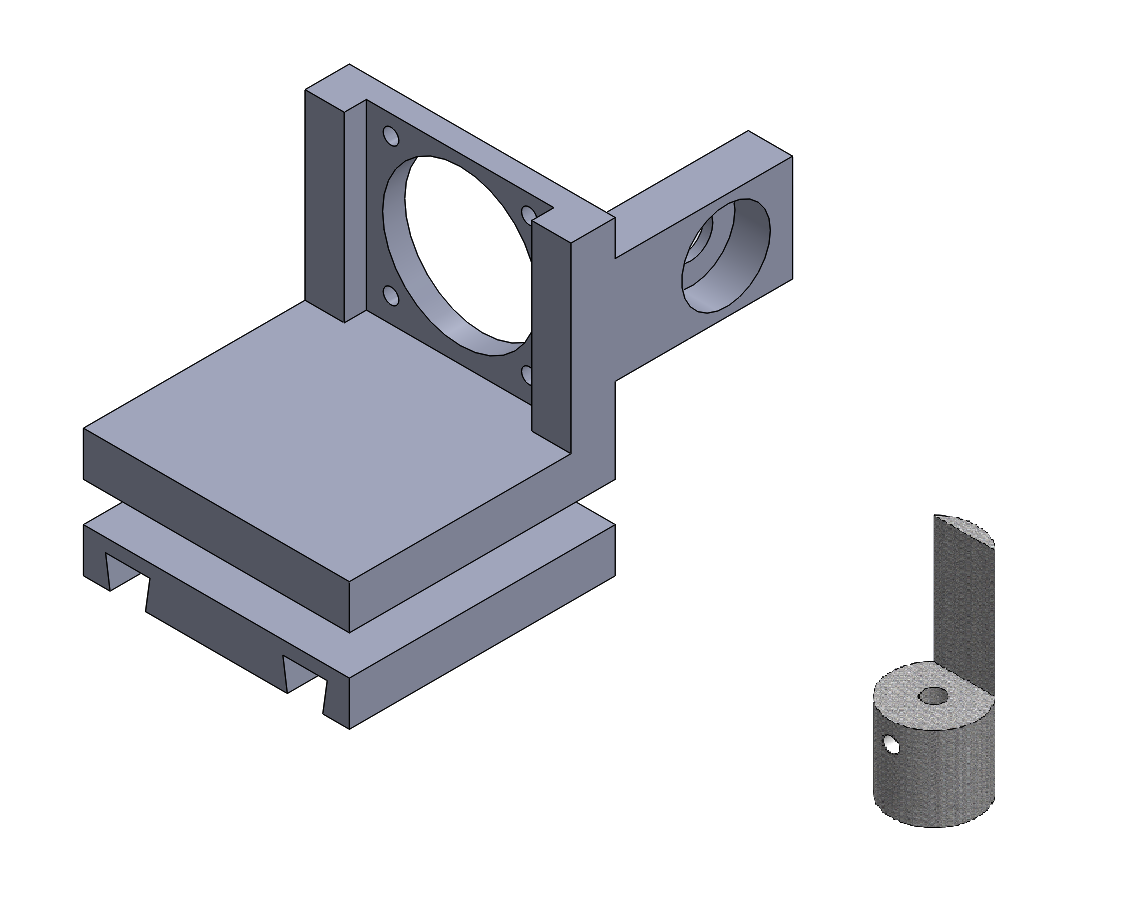
\includegraphics[width=0.65\textwidth]{fig/perfilador/soporte_v3}
\caption{Vistas tridimensionales del soporte, con el ensamble en un posible Cage}
\label{fig:perfilador/soporte_v3}
\end{figure}

La desventaja de este soporte es que es complicado, y hasta imposible por el tamaño del motor, usarlo en altura o poder medir en otro eje. De esta forma se diseño un modelo, visible en la figura \ref{fig:perfilador/soporte_v4}, alrededor de un motor de menores dimensiones, en este caso un NEMA 8 

\begin{figure}[H]
    \centering
    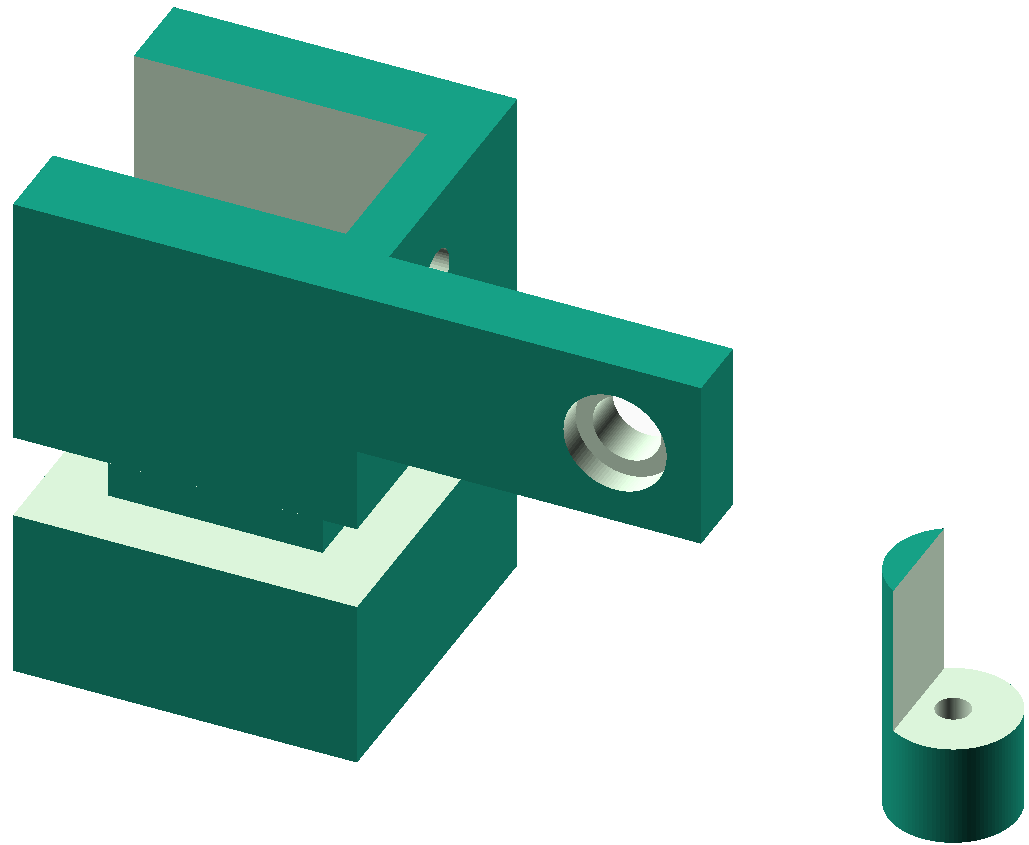
\includegraphics[width=0.4\textwidth]{fig/perfilador/soporte_v4}
    \caption{Vistas tridimensionales del soporte más el tambor de referencia}
    \label{fig:perfilador/soporte_v4}
\end{figure}

Este soporte tiene las ventajas de la anterior prototipo, como ser fácil colocación en la mesa óptica y con el motor encastrado para no tener mediciones erroneas. A su vez con un tornillo pasante en el centro del soporte es fácil de atornillar a cualquier soporte en altura o perpendicular para hacer mediciones en otros setups. El tamaño lateral al eje del motor está determinado por el tamaño del tambor, y por el tamaño del fotodiodo, pero se puede todavía achicar más en iteraciones siguientes.

\subsection{Electrónica de adquisición}

Como se busca al sistema lo más autónomo posible,  se necesita tener una electrónica con capacidad de mover el motor y medir el sensor de forma simultánea, y finalmente transmitir lo medido a una computadora. Esto implica que debemos construir un sistema embebido, y la mejor opción, si no la única viable, es utilizar un microcontrolador. 

\subsubsection{Controlador del motor}
Respecto al movimiento del motor, se utilizó un circuito integrado Pololu A4988\cite{pololu}, basado en Allegro A4988, que permite mover motores hasta 1$\,$A por fase y ejecutar pasos separados mínimamente por 1$\,\mu$s, más de lo necesario para el motor elegido, ya que representa una velocidad de rotación de 500RPS. Este integrado resuelve el control de corriente de las fases del motor, independiente de la tensión de la fuente. Es más permite setear el umbral de la corriente por un potenciometro, para aumentar el torque en caso de hacer microstepping. Como limitación a la tensión de entrada se necesita un mínimo de 8V, pero no es una limitación muy fuerte sobre la fuente; se usa una fuente de notebook que entrega 2A y 19V, a la cual ni es necesario filtrarla.

\subsubsection{Microcontrolador}
Respecto al microcontrlador, el laboratorio tenía disponible una placa Arduino\cite{arduino} UNO, que permite resolver la programación y la integración en proyectos de robótica o embebidos de forma simple para el usuario; se programa por USB y tiene un lenguaje de programación de alto nivel, en este caso un subconjunto de C++, y muchas librerías creadas por la comunidad para diversas aplicaciones.

Lamentablemente al mover el motor paso a paso y adquirir la señal analógica del fotodiodo al mismo, se encontró una limitación importante en la memoria RAM del Arduino UNO, de 2KiB. Este tamaño de memoria no es suficiente para guardar los datos de una vuelta, ya que solo se pudo guardar hasta 128 puntos (en este caso tiempo en microsegundos y tensión en bits del ADC), y se necesita guardar como mínimo 200 puntos o más si se usa microstepping. Es necesario medir una vez por paso, ya que de esta forma se tiene un disparo o trigger razonable para la adquisición analógica, aunque se podría medir una vez cada un múltiplo de pasos. 

Obviamente, se podría haber optado por medir 128 datos, pero al observar la transición para el haz de prueba se concluyó que esa cantidad de datos era insuficiente para conmensurar la transición con la precisión buscada; en este caso se observan 5 datos en una transición de un motor girando a 10RPS.

En la primera aproximación al control del motor, al transmitir los datos adquiridos se bloqueaba el movimiento del motor, ya que el tiempo consumido en esta transmisión es mayor al tiempo entre pasos. Para resolver esto, se utilizó la funcionalidad de PWM, Pulse Width Modulation, que consiste en una señal cuadrada con ancho de pulso variable (que para esta aplicación se usó un ciclo de trabajo del 50\%), con una frecuencia fija. Esta señal está generada por las interrupciones del microcontrolador, y no son alteradas por la transmisión de datos por el puerto USB.

Sin embargo para el Arduino UNO no es fácil de asignar la frecuencia de trabajo del PWM en cada pin, para lo cual es necesario cambiar detalles internos del microcontrolador.

Debido a todas estas limitaciones, se buscó un microcontrolador con mayor velocidad y más memoria RAM compatible con la plataforma Arduino, ya que se requiere que sea fácil de programar.

La placa de desarrollo Teensy v3.2\cite{teensy} cumplía con todo lo pedido; este dispositivo tiene una velocidad de procesador por defecto de 72MHz, y alcanza 96MHz, y 64KiB de RAM, tal vez un poco sobredimensionado para la aplicación. El pinout, es decir la funcionalidad de cada pin, se ve en la figura \ref{fig:circuito/teensy}. Además la plataforma de desarrollo tiene disponible un mecanismo simple para alterar la frecuencia del PWM, permitiendo generar aceleraciones y alcanzar velocidades más altas del motor fácilmente.

Probando la transmisión por USB de este microcontrolador se llegó al límite de 1200 datos transmitidos cada 0,5s. Este límite está impuesto por la velocidad de microcontrolador y la computadora utilizada, ya que el protocolo de transmisión está hecho por software.

Para aún mejorar más la portabilidad del instrumental, se buscó un integrado capaz de transmitir por radiofrecuencia, en especial WiFi ya que se sabe que se implementan protocolos TCP que manejan de forma eficiente paquetes grandes y puede mejorar aún más la velocidad de transferencia de datos.

El primer integradro con WiFi probado se denomina NodeMCU, que tiene la particularidad de ser programable por lenguajes de muy alto nivel, como es Lua o Python. Lamentablemente este integrado no tiene la velocidad de adquisición de datos necesaria, además de tener una documentación pobre, por lo que fue rápidamente descartado.

Finalmente, se hicieron pruebas con el microcontrolador Particle Photon\cite{particle_photon} (de Particle.io), que se puede ver en la figura \ref{fig:circuito/photon} (junto al lado del pinout del $\mu$C Teensy para comparar rápidamente). Este microcontrolador tiene integrado un circuito Broadcom BCM43362, que probee WiFi clase b/g/n, con un microcontrolador Freescale STM32F205 ARM Cortex M3 a 120MHz, con 128KB de RAM; de esta forma es microcontrolador Teensy, con el doble de memoria RAM, más todo el circuito de comunicación WiFi. 

 Respecto a la programación, el microcontrolador se programa en C++ enteramente, lo que hace mucho más simple el uso de librerías y código fuente de la comunidad. No solo eso, el sistema puede, y además se recomienda, ser programado desde Internet y además permite con una interfaz simple de usar publicar datos medidos en la nube cada 1s. Este microcontrolador está especialmente pensando para la Internet of Things, que busca automatizar y medir todos los procesos de los diferentes aparatos en una casa o en una oficina (como se el aire acondicionado, la heladera, etc).

\begin{figure}[H]
    \begin{subfigure}[b]{0.45\textwidth}
        \centering
        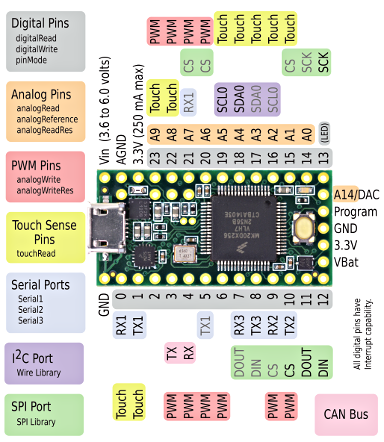
\includegraphics[width=0.8\textwidth]{fig/circuito/teensy32_front_pinout}
        \caption{Pinout del $\mu$C Teensy. Dispone de muchas entradas/salidas digitales, varias entradas analógicas y una salida analógica}
        \label{fig:circuito/teensy}
    \end{subfigure}
    \begin{subfigure}[b]{0.45\textwidth}
        \centering
        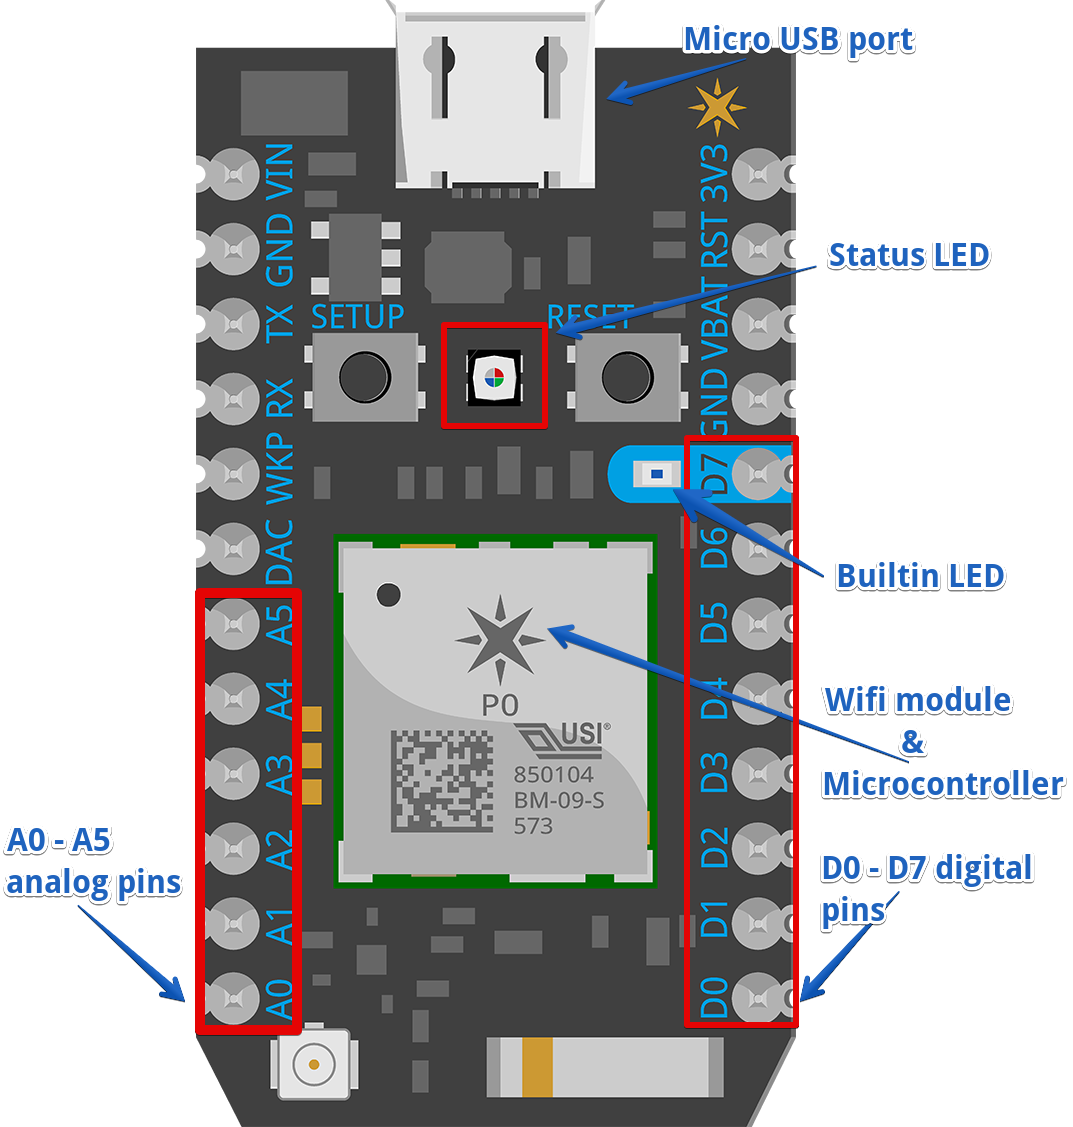
\includegraphics[width=0.8\textwidth]{fig/circuito/photon}
        \caption{Pinout del $\mu$C Photon. Destacable el diseño simplificado del pinout, además del LED RGB y el módulo WiFi}
        \label{fig:circuito/photon}
    \end{subfigure}
    \caption{Microcontroladores utilizados comparado en su capacidades de entradas/salidas}
\end{figure}

\subsubsection{Amplificación de la señal}

El sensor utilizado corresponde a un fotodiodo  FDS010\cite{fds010} de Thorlabs, que en su hoja de datos determinar que se debe polarizar en inversa y utilizar una resistencia de carga. Un fotodiodo es modelado como una fuente de corriente dependiente de la luz incidente, por lo que es necesario transformar esa salida en una tensión medible. También se constató que la capacitancia del fotodiodo utilizado no altere la medición; en particular, este fotodiodo es capaz de responder en el orden de los nanosegundos, por lo que permite utilizarlo sin problemas.

Sin embargo, si se mide la corriente del fotodiodo en una resistencia de carga se observa un desajuste de la función error a la señal medida, como se ve en la figura \ref{fig:circuito/desajuste}

\begin{figure}[H]
    \centering
    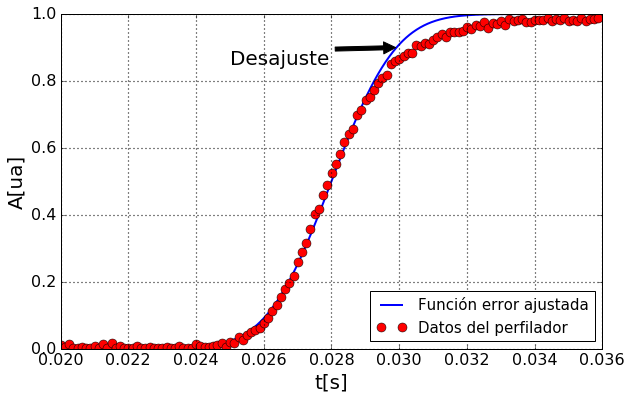
\includegraphics[width=0.5\textwidth]{fig/perfilador/labo6/fit_data_labo6_anotado}
    \caption{Medición de la tensión en una resistencia de carga producida por la corriente del fotodiodo al perfilar un haz}
    \label{fig:circuito/desajuste}
\end{figure}

Este problema proviene de la resistencia de carga utilizada, que debido que la corriente del fotodiodo es muy pequeña, debe ser de un valor razonablemente grande. Esto produce que el circuito se comporte como un filtro RC pasa bajos, por lo que al tener un cambio brusco en la intensidad de luz, la corriente no responderá igual de rápido (al perder componentes en frecuencia). 

Para solucionar esto, se propone la construcción de un amplificador de transimpedancia, es decir un amplificador de corriente en tensión, por medio de un amplificador operacional. Este integrado permite con crear circuitos complejos con muy pocas componentes, la mayoría pasivos, como en este caso una resistencia en la rama de retroalimentación; en la figura \ref{fig:circuito/tia} se ve el esquema del amplificador

\begin{figure}[H]
    \centering
    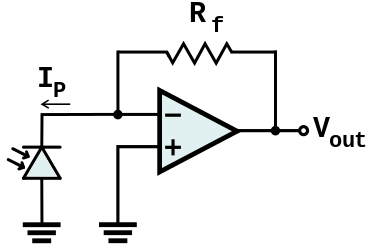
\includegraphics[width=0.35\textwidth]{fig/circuito/amp/TIA}
    \caption{Esquema del amplificador de transimpedancia implementado}
    \label{fig:circuito/tia}
\end{figure}

El operacional utilizado es el LM358, que tiene la ventaja de poder funcionar con fuente simple. De esta forma no es necesario tener tensiones negativas, pero si uno observa la hoja de datos del integrado se encuentra que no es rail-to-rail. Es decir la tensión máxima de salida no llega a a excursionar hasta la tensión de alimentación y además no es posible obtener una señal de salida con valor nulo (igual a 0V).

Para calibrar este amplificador se lo alimenta con una señal cuadrada, en este caso de corriente, para observar la respuesta en frecuencia y una señal triangular para observar la linealidad del sistema. Estas calibraciones se disponen en la figura \ref{fig:circuito/amp/transicion_escalon} y \ref{fig:circuito/amp/rango_lineal}.

\begin{figure}[H]
    \begin{subfigure}[b]{0.5\textwidth}
        \centering
        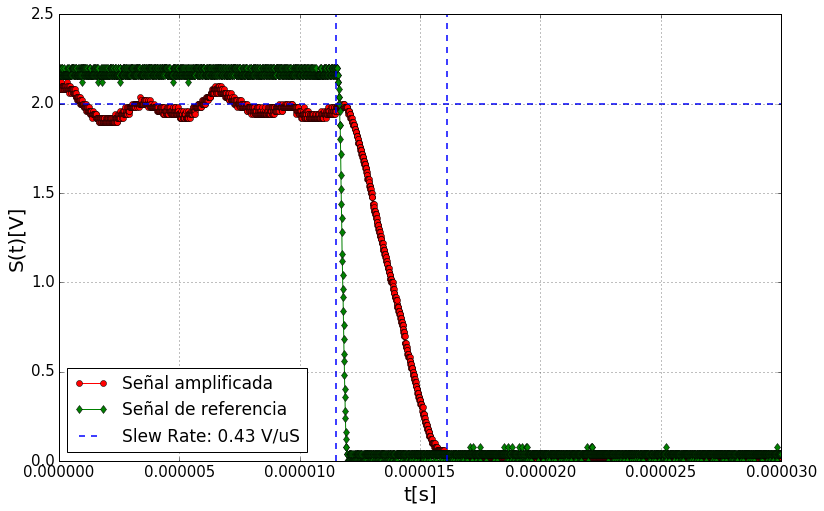
\includegraphics[width=0.8\textwidth]{fig/circuito/amp/transicion_cuadrada}
        \caption{Respuesta al escalón}
        \label{fig:circuito/amp/transicion_escalon}
    \end{subfigure}
    \begin{subfigure}[b]{0.5\textwidth}
        \centering
        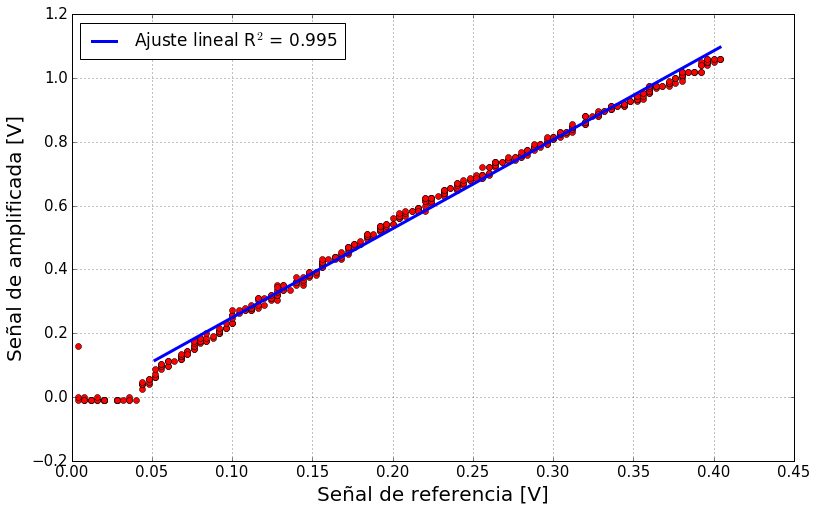
\includegraphics[width=0.8\textwidth]{fig/circuito/amp/rango_lineal}
        \caption{Respuesta a una señal lineal}
        \label{fig:circuito/amp/rango_lineal}
    \end{subfigure}
    \caption{Calibraciones del amplificador de transimpedancia implementado}
\end{figure}

De la figura \ref{fig:circuito/amp/transicion_escalon} se deduce que el \emph{slew rate}, o tiempo de reacción del integrado, es de 0,4$\,$V $\mu$s$^{-1}$, que es hasta 4 veces más rápido de lo necesario según lo que se observa en las mediciones preliminares. Aún a una velocidad de 30RPS las transiciones se harían a 0,2 $\,$V $\mu$s$^{-1}$, por lo que el amplificador operacional está sobredimensionado.

Respecto al rango lineal se observa no es posible acusar corrientes muy grandes ni corrientes nulas, pero el rango lineal es bastante amplio para las mediciones. En general la corriente oscura imposibilita generar mediciones de corriente nula, lo que permite usar satisfactoriamente este amplificador para la aplicación.

Finalmente la adquisición que se logró con el amplificador está plasmada en la figura \ref{fig:circuito/amp/perfilacion_ajuste}, donde se puede observar que la señal es ajustada correctamente por la función error, detalle que se esperaba que sucediera, solucionando el problema para el cual el amplificador fue construido exitosamente

\begin{figure}[H]
    \centering
    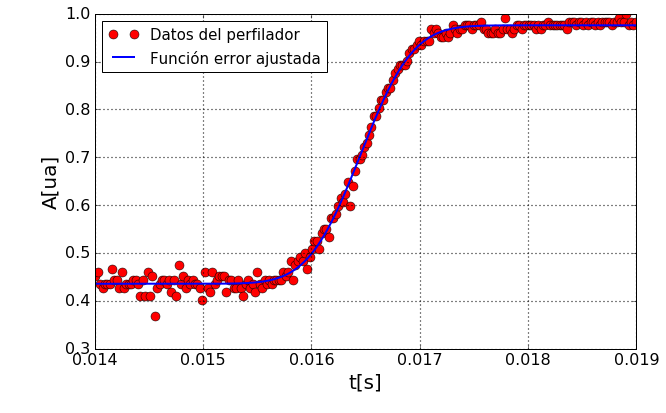
\includegraphics[width=0.5\textwidth]{fig/perfilador/fit_data_plastico_subida}
    \caption{Señal del fotodiodo al perfilar amplificada, con un ajuste de la función error}
    \label{fig:circuito/amp/perfilacion_ajuste}
\end{figure}
Cabe destacar que al amplificar la señal, también se amplifica el ruido de esta y la corriente oscura del fotodiodo, aún cuando esta bastante pequeña ya que no está polarizado en inversa, lo que hace la señal (como se ve en la figura \ref{fig:circuito/amp/perfilacion_ajuste}) más ruidosa. Sin embargo, la relación señal ruido es más que satisfactoria para la aplicación.

\subsubsection{Software el microcontrolador}
El circuito final fue implementado una placa de 5x5$\,$cm, junto con una fuente reductora de tensión para alimentar al microcontrolador a partir de la tensión del fuente de notebook, lo que permite utilizarlo fácilmente en la mesa óptica del laboratorio. El esquemático y el circuito impreso están liberados para el uso de la comunidad en el proyecto SOMA, y se encuentran en el apéndice.

El software del microcontrolador ya está pensando para el perfilador y polarimetro, midiendo la señal del fotodiodo solo cuando la computadora le manda la señal (es decir por un disparo externo), de forma sincrónica utilizando un delay proporcional al tiempo entre pasos del motor. Finalmente se manda toda la señal por protocolo Telnet, que no es más que un mensaje TCP con el texto del mensaje (en este caso los datos). En este caso al conectarse el cliente Telnet, la computadora, el microcontrolador nota la conexión y empieza a mandar la señal, y al final cierra la conexión; de esta forma no es necesario mandar ninguna señal del inicio, solamente conectarse a con la IP y el puerto TCP con un cliente Telnet.

El microcontrolador es capaz de mandar hasta 4000 datos cada 0,1s aproximadamente, lo que la velocidad de adquisición queda totalmente determinada por el motor; 4000 datos representan 20 vueltas del motor, o 40 transiciones, por lo que la velocidad de transferencia de datos es de 200 vueltas por segundo.

\subsection{Adquisición de datos}

Ya definido y construido el circuito del perfilador, en la computadora es necesario definir el software para obtener los datos crudos de la medición del fotodiodo, y finalmente deducir información útil del perfil. 

Para determinar el tamaño del haz, se propuso ajustar los datos asumiendo que el perfil es gaussiano. Como la medición de la corriente del fotodiodo corresponde a la integral de la intensidad del haz, el ajuste por cuadrados mínimos será de una función error, representada en la figura \ref{fig:err_function}, donde el ancho medio se corresponde con la mitad del tamaño del haz.

Para poder encontrar el tamaño del haz a partir de varias transiciones, que provienen de la medición efecutada por la electrónica, es necesario definir la sección del gráfico o ventana temporal donde ajustar la función error. Para eso, se procede a obtener una frecuencia característica a partir de una transformada de Fourier y luego se buscan los puntos más cercanos al valor medio de la señal, por medio de un filtro gaussiano para detección de bordes. Finalmente se ajusta la función error dentro de la ventana temporal definida por un cuarto del tiempo característico (la inversa de la frecuencia característica) centrada los puntos más cercanos al valor medio. 

Es rescatable que todo este algoritmo procede de forma automático, solo asumiendo que los datos tienen las transiciones esperadas, y en caso de no tener una señal de esa forma se acusa un error, del cual se recupera y sigue midiendo.

Respecto al polarimetro, se ajusta una función coseno cuadrado y si el ajuste es exitoso se obtiene el coeficiente $\alpha$ (ecuación \ref{eq:polarizacion/alpha}), con los valores máximos y minimos del ajuste. De esta forma el software del polarimetro es muchisimo más simple que la del perfilador, lo que permitió cearlo rápidamente.

Todo el programa de obtención de los datos del microcontrolador y el acondicionamiento de datos se programó con Python v3.5, usando librerías Numpy v1.10.1, Scipy v0.16.1, Pandas v0.17 y Matplotlib v1.5.0, aunque funciona en versiones anteriores de la rama v3.x de Python. Este entorno, con la documentación, es libre en su totalidad, y además el software implementado está documentado para su posterior uso. 

El programa final de adquisición se le construyó una interfaz gráfica para poder ser más fácil de utilizar. Esta interfaz fue creada en PyQT, y es de muy fácil portado a todos los sistemas operativos usuales.

\subsection{Polarimetro}

Con la electrónica de adquisición y control del motor desarrollado para el perfilador, se construyó un polarímetro utilizando el concepto visto en la figura \ref{fig:polarimetro/esquema}. Para ello se consideró utilizar unos engranajes, uno de ellos motorizado y otro con la lámina polarizadora, y un fotodiodo midiendo la intensidad que atravieza la lámina.

El soporte diseñado para los engranajes se puede observar en la figura \ref{fig:polarimetro/soporte}, junto con los engranajes en la figura \ref{fig:polarimetro/engranajes}. El polarimetro funciona rotando el engranaje menor y el engranaje mayor tiene la lámina polarizadora pegada o colocada dentro de eje de dicho. El fotodiodo tiene un soporte detrás de la pieza, midiendo la intensidad del haz que atravieza la lámina polarizadora.

\begin{figure}[H]
    \begin{subfigure}{0.45\textwidth}
        \centering
        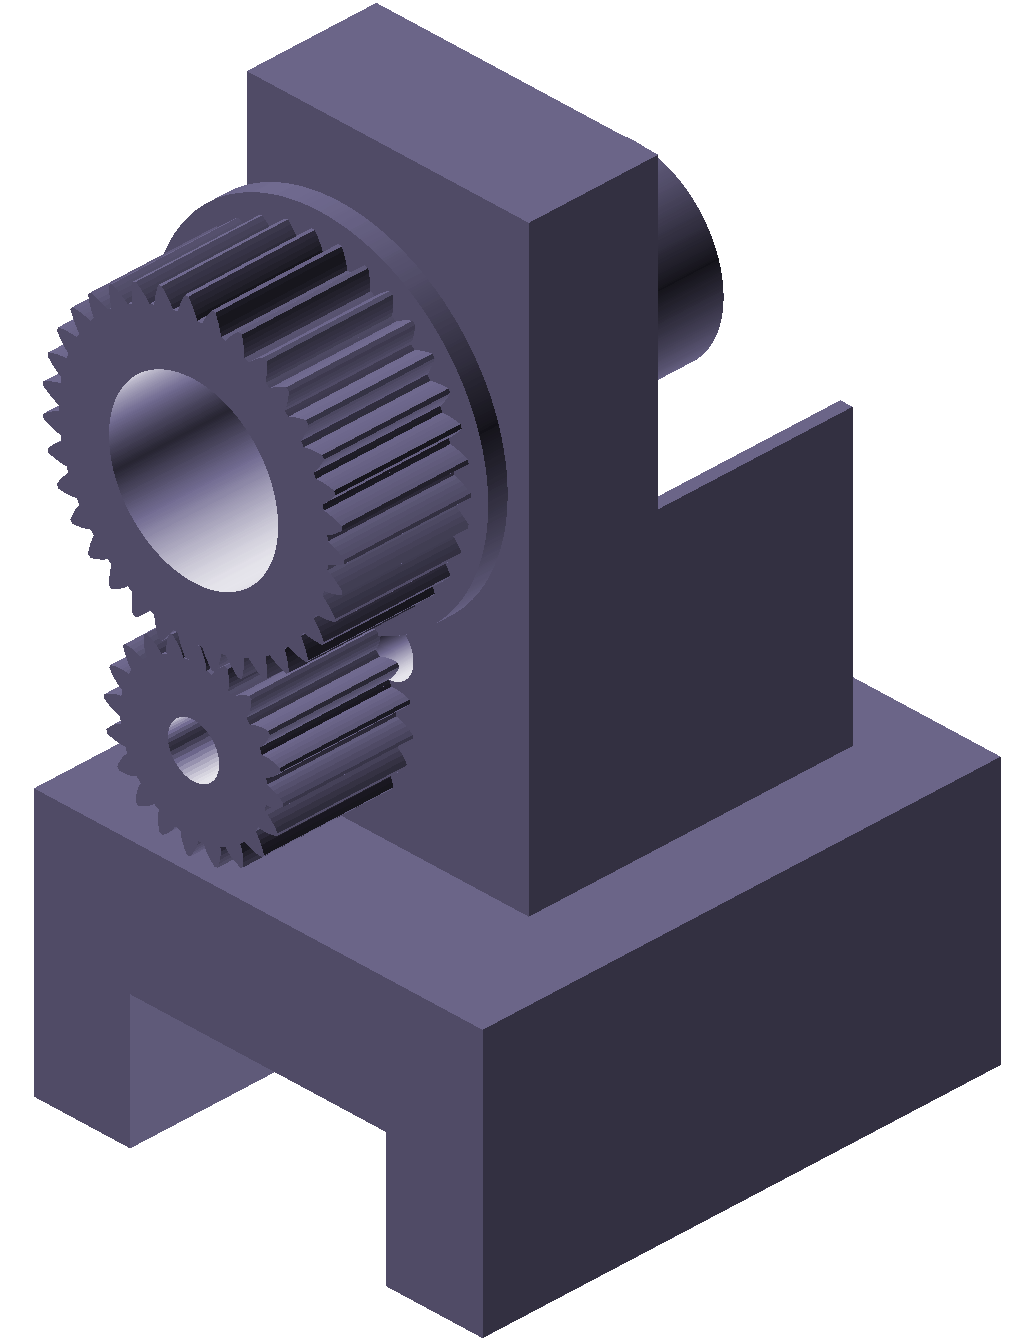
\includegraphics[width=0.7\textwidth]{fig/polarimetro/soporte_all}
        \caption{Polarímetro armado, sin el motor ni el fotodiodo}
        \label{fig:polarimetro/soporte}
    \end{subfigure}
    \begin{subfigure}{0.45\textwidth}
        \centering
        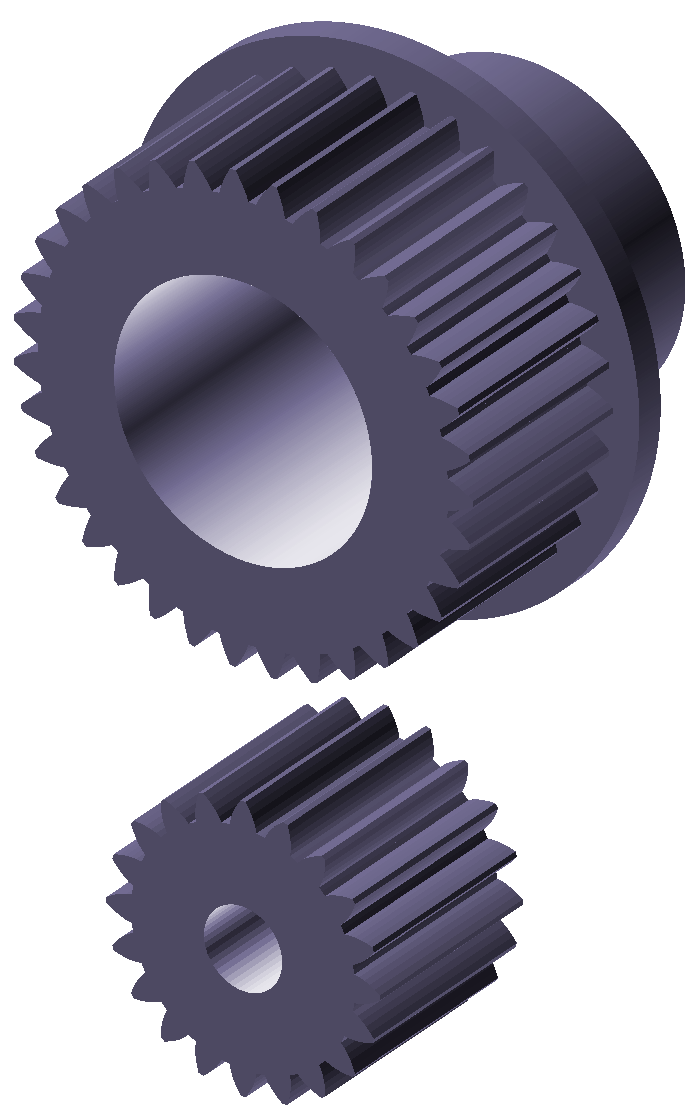
\includegraphics[width=0.7\textwidth]{fig/polarimetro/engranajes}
        \caption{Engranajes}
        \label{fig:polarimetro/engranajes}
    \end{subfigure}
    \caption{Vistas tridimensionales del polarímetro}
\end{figure}

Debido a imperfecciones del movimiento, el engranaje grande puede salirse del soporte, por lo que se le agregó una arandela (impresa) para limitar el movimiento en esa dirección. 

Finalmente, luego de imprimirse se debieron hacer algunos ajustes para mejorar la mecánica, lijando las superficies rotante. Esto también se debe a que en las impresiones 3D siempre se agrega material de soporte para que no se deforme mientras se imprime la pieza.

Igualmente, los problemas mecánicos persisten, por lo que se baja la velocidad (aumentando el torque) a 10RPS. A esta velocidad los engranajes giran sin problemas de forma continua, y además no mella la velocidad de adquisición de polarización. Hay que recordar que no se busca medir en tiempo real, solamente superar al mecanismo manual, que puede tardar entre 5 a 10 minutos por medición.

El soporte no está pensando explicitamente pensando para ser ubicado en altura, pero al ser de pequeñas dimensiones es factible crear con elementos del laboratorio una base con altura arbitraria. Además el soporte puede entrar fácilmente en un Cage de Thorlabs.


    \section{Resultados}
        Implementado los diseños, el perfilador se utilizó para medir el haz en el SPIM, como prototipo de cualquier setup del laboratorio.

\subsection{Mediciones preliminares con el perfilador}
Los primeros prototipos del perfilador, en el marco de Laboratorio 6, se utilizaron para medir el haz de un laser HeNe a la salida de una fibra óptica Thorlabs F220FC-A\cite{thorlabs_fc}, con un tamaño del haz en plano focal nominal de 2$\,$mm en ambos ejes y una divergencia de 0.020$^\circ$. Se hicieron mediciones manuales de este haz para constrastar y calibrar el perfilador.

Los datos medidos están en la figura \ref{fig:perfilador/calibracion_preliminar}, donde el error de la intensidad fue estimado con la variación de la intensidad y el error acusado por el fabricante del instrumental. El error en las abscisas está graficado, pero es despreciable.

\begin{figure}[H]
    \centering
    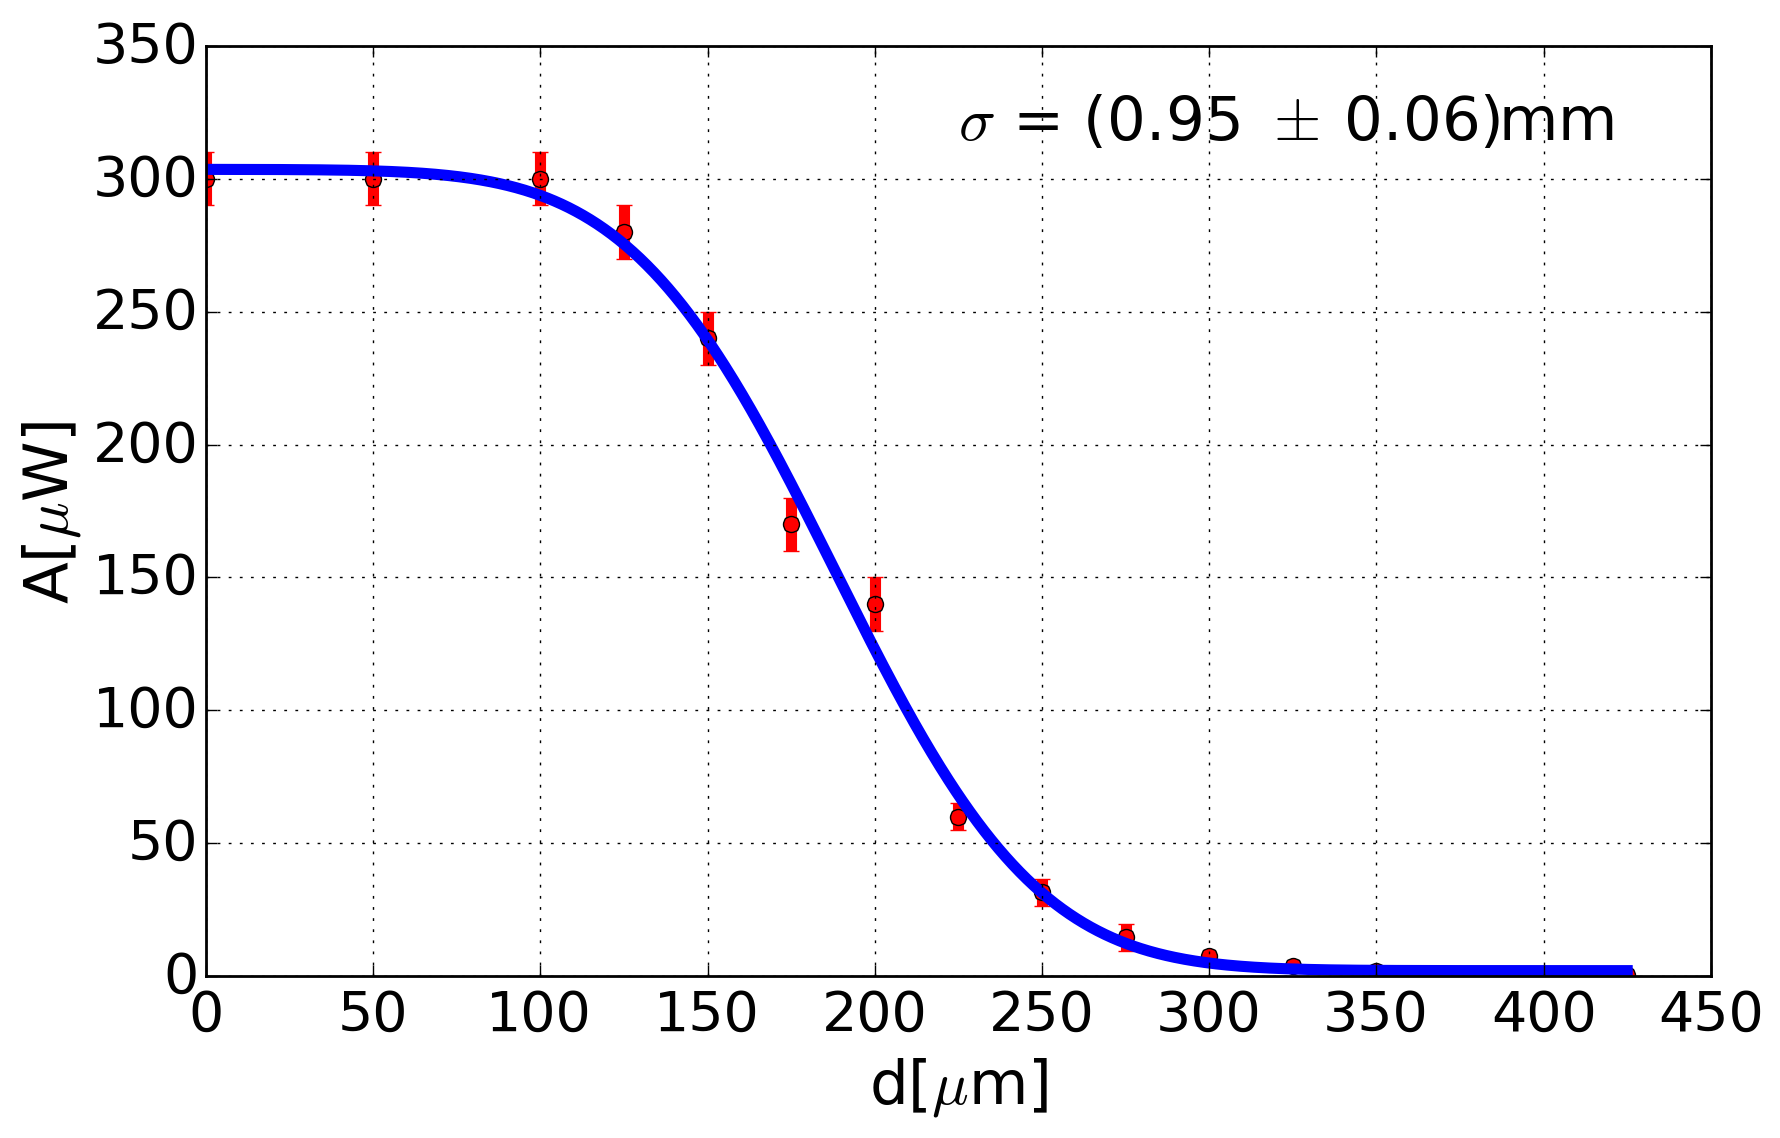
\includegraphics[width=0.4\textwidth]{fig/perfilador/calibracion_preliminar}
    \caption{Perfilación del haz utilizado de forma manual, con el ajuste efectuado. El error en la posición está graficado pero es despreciable}
    \label{fig:perfilador/calibracion_preliminar}
\end{figure}

Podemos ver que esa figura también se agregó el ajuste de la función error. De ese ajuste, el único parámetro que interesa es el ancho medio, que es la mitad del tamaño del haz, ya que la amplitud depende fuertemente del sensor y la amplificación utilizada. Tampoco es necesario saber, para las aplicaciones del laboratorio, la intensidad máxima absoluta del haz.

El ajuste efectuado acusa un valor de tamaño medio de $\sigma = (0,95\pm0,06)\,$mm, y recordemos que del colimador utilizado sale un haz con un tamaño de 2$\,$mm en el plano focal, por lo que el valor acusado por el fabricante parece estar bien tabulado. Este valor de $\sigma$ representa la calibración con la que se contrastará el perfilador.

En la figura \ref{fig:perfilador/preliminar_fit} se puede ver los datos obtenidos del microcontrolador.

\begin{minipage}[c]{0.55\textwidth}
\begin{figure}[H]
    \centering
    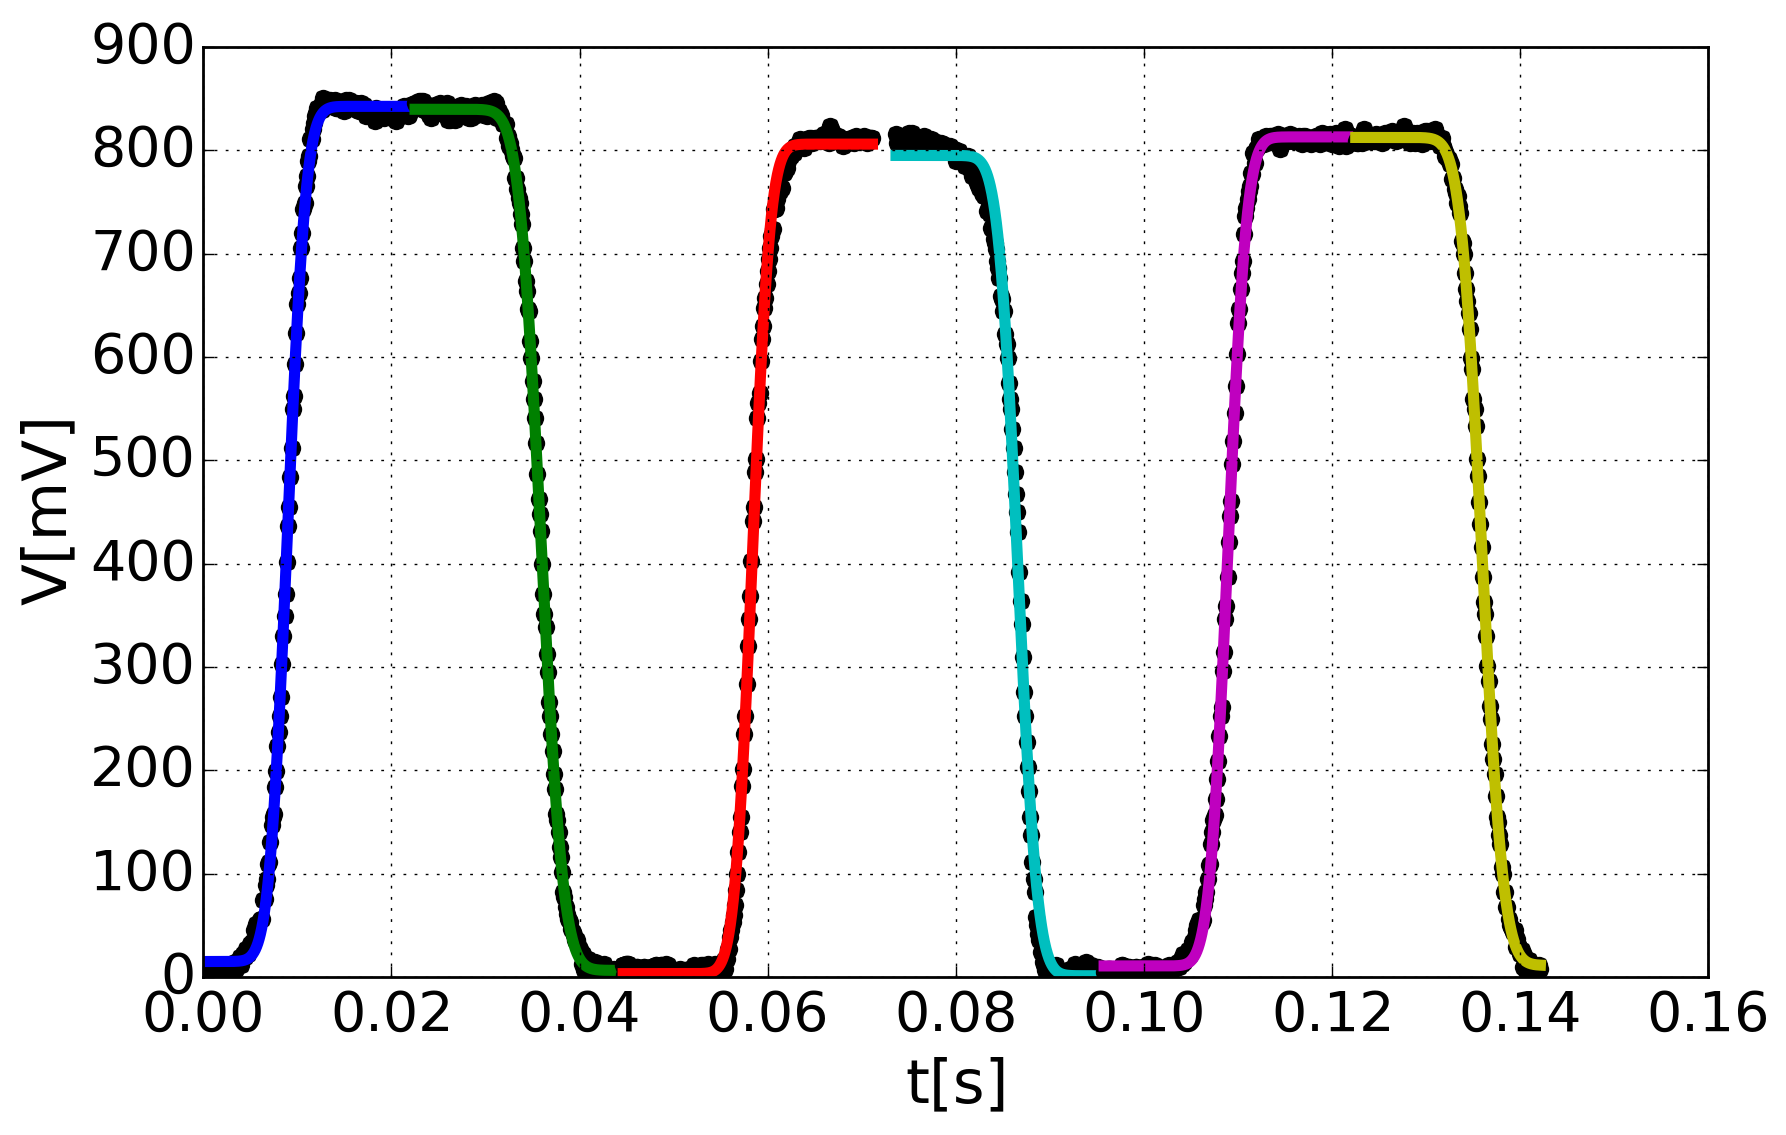
\includegraphics[width=0.8\textwidth]{fig/perfilador/preliminar_fit}
    \caption{Datos medidos con el perfilador a la salida del colimador del SPIM, con las transiciones separadas y ajustadas}
    \label{fig:perfilador/preliminar_fit}
\end{figure}
\end{minipage}
\begin{minipage}[c]{0.35\textwidth}
    \begin{table}[H]
        \centering
        \begin{tabular}{c|c}
            Perfil & $\sigma[\text{mm}]$ \\ \hline
            1 & 1,95 $\pm$ 0,21 \\
            2 & 2,34 $\pm$ 0,24 \\
            3 & 1,88 $\pm$ 0,21 \\
            4 & 2,05 $\pm$ 0,24 \\
            5 & 1,97 $\pm$ 0,21 \\
            6 & 2,27 $\pm$ 0,24 \\
        \end{tabular}
        \caption{}
        \label{tbl:perfilador/preliminar_fit}
    \end{table}
\end{minipage}
\\ \\
Se observa diferencias entre las diferentes transiciones, en especial las que se esperan que sean idénticas (ya que el tambor obtura en el mismo plano el haz para obtenerlas), de hasta 0,2$\,$mm, lo que significa un error de 20\%. No solo eso, se observa una discrepancia del 100\%, es decir un 1$\,$mm, con la calibración (y el tamaño del haz tabulado por el fabricante del colimador). 

Esto lleva a diseñar un tambor metálico, como ya se mencionó, y nuevos diseños del soporte del perfilador.

\subsection{Calibración y mediciones del perfilador}
Habiendo hecho mediciones con los primeros prototipos en Laboratorio 6, se pasó a medir el perfil, en Laboratorio 7, con el tercer y cuarto prototipo (\ref{fig:perfilador/soporte_v3} y \ref{fig:perfilador/soporte_v4}) con el tambor de metal y una nueva impresión en plástico, esta vez a la salida de una colimador de fibra Thorlabs F280\cite{thorlabs_fc} (con un diametro de haz nominal de 3,3$\,$mm en ambos ejes). 

Las mediciones efectuadas, en este caso en el foco del colimador mencionado, se pueden observar en las figuras \ref{fig:perfilador/spim_foco}, con un acercamiento en \ref{fig:perfilador/spim_foco_zoom}

\begin{figure}[H]
    \begin{subfigure}[b]{0.5\textwidth}
        \centering
        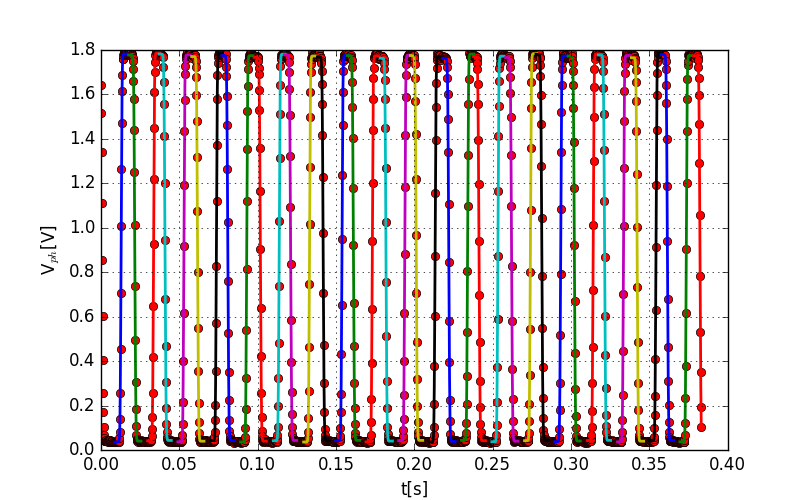
\includegraphics[width=\textwidth]{fig/perfilador/spim_foco}
        \caption{Conjunto de datos obtenidos en una petición del software de adquisición, con los ajustes efectuados}
        \label{fig:perfilador/spim_foco}
    \end{subfigure}
    \begin{subfigure}[b]{.5\textwidth}
        \centering
        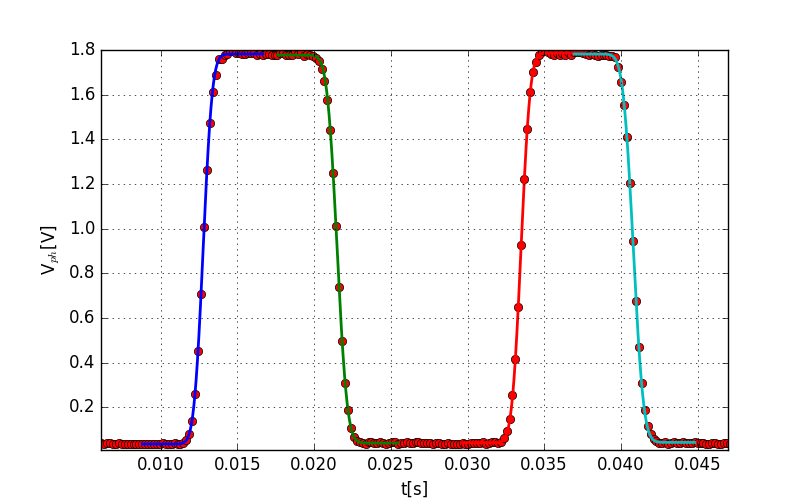
\includegraphics[width=\textwidth]{fig/perfilador/spim_foco_zoom}
        \caption{Zoom sobre la figura \ref{fig:perfilador/spim_foco} para observar las transiciones}
        \label{fig:perfilador/spim_foco_zoom}
    \end{subfigure}
    \caption{Datos obtenidos del perfilador en el foco del colimador F280FC-A}
\end{figure}

Al promediar cada perfil se obtiene que el haz mide $(3,03\pm0,15)\,$mm. Se observa una diferencia con el valor reportado por el fabricante, de 3,3$\,$mm, que se asocia a un error sistemático en la medición; puede ser por el fotodiodo utilizado, pero no se ha podido diferenciar. 

Para aseverar esta discrepancia, se hicieron mediciones manuales del perfil, que se ven en la figura \ref{fig:perfilador/spim_foco_manual}, donde queda en evidencia una discrepancia, pero las mediciones manuales y automática se solapan. Resta entender la discrepancia encontrada con el valor nominal expresado por el fabricante, ya que el tamaño del haz a la salida del colimador es un parámetro determinante del tamaño (y por ende de la precisión) del lightsheet del SPIM.

\begin{figure}[H]
    \centering
    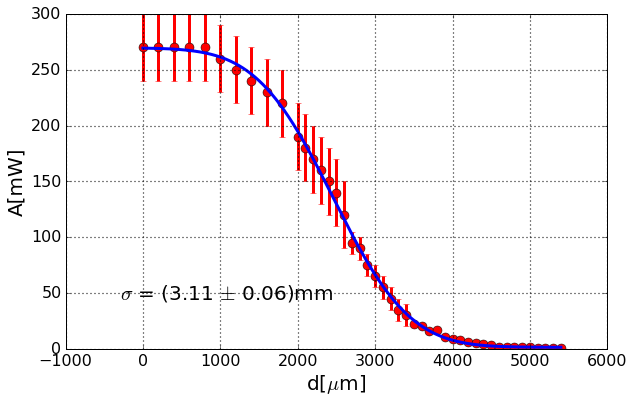
\includegraphics[width=0.55\textwidth]{fig/perfilador/calibracion_f280}
    \caption{Medición manual del perfil del haz para el colimador F280FC, con el ajuste de la función error}
    \label{fig:perfilador/spim_foco_manual}
\end{figure}

La ventaja del perfilador automático sobre la medición manual es la capacidad de realizar 40 mediciones en 0,4$\,$s como se ve en la figura \ref{fig:perfilador/spim_foco}, frente a una medición cada cinco minutos que puede lograr con un método manual, además de ser un sistema más simple de colocar y utilizar; depende del setup, puede llevar entre 10 a 15 minutos construir el perfilador manual y montarlo, mientras el perfilador automático en un par de minutos ya está midiendo. 

Para concluir las mediciones del perfilador, se midió el haz dentro del telescopio del SPIM, para observar la divergencia del haz. Estas mediciones está plasmadas en la figura \ref{fig:perfilador/spim_telescopio}, con los valores ajustados ya promediados (ya que se tienen dos tamaños de haces bien definidos) en la tabla \ref{tbl:perfilador/spim_telescopio}.

\begin{minipage}[c]{0.55\textwidth}
\begin{figure}[H]
    \centering
    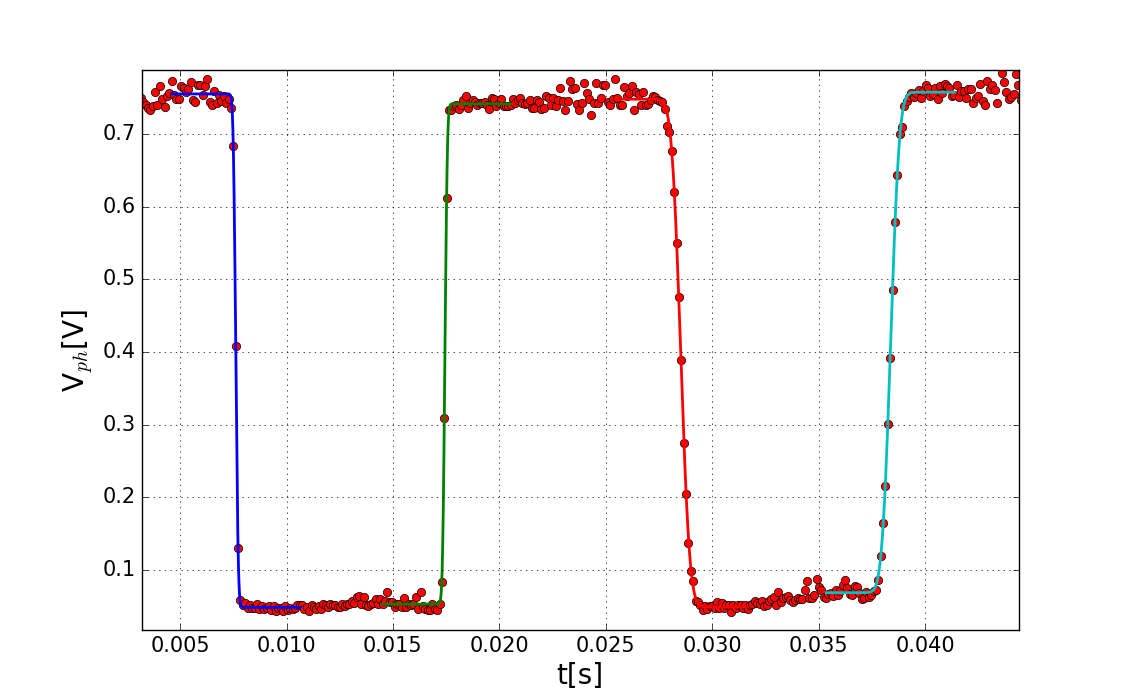
\includegraphics[width=\textwidth]{fig/perfilador/spim_telescopio}
    \caption{Datos medidos dentro del telescopio del SPIM, con las transiciones separadas y ajustadas}
    \label{fig:perfilador/spim_telescopio}
\end{figure}
\end{minipage}
%
\begin{minipage}[c]{0.35\textwidth}
    \begin{table}[H]
        \centering
        \begin{tabular}{c|c}
            Perfil & $\sigma[\text{mm}]$ \\ \hline
            1 & 0, 55$\pm$0,02  \\
            2 & 2,11$\pm$0,05 \\
        \end{tabular}
        \caption{Ajustes efectuados y promediados en la figura \ref{fig:perfilador/spim_telescopio}. Acá queda en evidencia la existencia de una divergencia del haz apreciable, considerando que entre obturaciones se observa el mismo perfil, no así entre desobturaciones}
        \label{tbl:perfilador/spim_telescopio}
    \end{table}
\end{minipage}
\\ \\

Al tener el mismo tamaño de haz entre dos obturaciones del tambor, cuando la señal es nula, pero no así entre desobturaciones, cuando la señal es máxima, se puede concluir que el perfilador está midiendo una divergencia del haz (recordar la figura \ref{fig:perfilador/corte_tambor} para tener noción de la perfilación).

Si este conjunto de mediciones lo ingresamos en la ecuación \ref{eq:perfilacion/gauss_divergence} podemos obtener la posición del foco y el ancho de cintura del haz en ese punto. De esta cuenta se obtiene dos soluciones, condensadas en la tabla \ref{tbl:perfilador/spim_telescopio_predicciones}.

\begin{table}[H]
        \centering
        \begin{tabular}{c|c|c}
            Solución & $z_0[\text{mm}]$ & $w_0[\text{mm}$] \\ \hline
            1 &  16,15 &  1,550$\times10^{-3}$  \\
            2 &  26,24 &  2,518$\times10^{-3}$\\
        \end{tabular}
        \caption{Prediciones de sobre el haz gaussiano a partir de los datos vistos en la figura \ref{fig:perfilador/spim_telescopio} y la ecuación \ref{eq:perfilacion/gauss_divergence}}
        \label{tbl:perfilador/spim_telescopio_predicciones}
\end{table}

Estas predicciones con consistentes con una perfilación con el foco dentro del tambor y con una perfilación con el foco fuera del tambor con el haz convergiendo. Ambas soluciones se explican conociendo el funcionamiento del telescopio para haces gaussianos, por lo que las mediciones verifican la hipotesis de la medición de la divergencia del haz.

Es preciso recordar que esta medición se hizo solo en un punto del espacio, y con ello se pudo observar la divergencia del haz. Si el camino óptico es ordenes de magnitud más grande que el tamaño del tambor, se deben hacer mediciones a varias distancias para poder observar de forma cabal la divergencia.

\subsection{Mediciones del polarímetro}

Las mediciones con el polarímetro fueron determinadas por la inicial calibración del material polarizante, en este caso una lámina polarizadora plástica, y luego por mediciones antes y después de la fibra del SPIM. Estas mediciones, como ya mencionamos, buscan determinar si la fibra óptica es capaz de mantener la polarización del haz incidente.

Para medir correctamente con el polarímetro, se tiene que conocer la matriz de transición de la lámina polarizadora, ya que representa la transmitancia de cada componente. Para esto, se crearon dos polarizadores rotantes con el material del polarizador y se midió la intensidad de un haz polarizado, proveniente de un láser HeNE Melles Griot 05-LGP-193, atravezando un conjunto de estados de alineación. Estas mediciones están condensadas en la tabla \ref{tbl:polarimetro/calibracion}


\begin{table}[H]
    \centering
    \begin{tabular}{c|c}
        Alineación  & P[$\mu$W] \\ \hline
        Sin láminas & 715 $\pm$ 5  \\
        Intensidad máxima, 1 lámina  & 330 $\pm$ 10 \\
        Intensidad mínima, 1 lámina  & 1,5 $\pm$ 0,1 \\
        Intensidad máxima, 2 láminas, una alineada & 160 $\pm$ 5 \\
        Intensidad minima, 2 láminas, una alineada & 0,7 $\pm$ 0,1 \\
    \end{tabular}
    \caption{Mediciones de calibración de lámina polarizadora}
    \label{tbl:polarimetro/calibracion}
\end{table}

De estas mediciones se deducen que la matriz de transferencia tiene la siguiente forma
\begin{equation}
    \begin{pmatrix} 0.461 & 0 \\ 0 & 2,097\times10^{-3} \end{pmatrix}.
\end{equation}

En esta matriz están condesados algunos detalles del polarizador. La transferencia en el eje principal es de 46,1\%, lo que representa una perdida importante de potencia lumínica, y la transferencia en el eje perpendicular no es exactamente cero, lo que implica que un haz polarizado lineal generará una señal coseno cuadrado más un offset. Esta señal puede eliminarse si se conoce la intensidad del haz al llegar al polarizador. 

Esta imperfección del polarizador genera problemas solo si se trata de dicernir una polarización lineal de una elíptica, pero las demás polarizaciones quedan bien definidas. De esta forma, se pudieron hacer mediciones con esta lámina, ya que se busca minimamente separar una polarización aleatoria de una polarización definida.

Finalmente se midió la polarización antes de la fibra del SPIM, y después del colimador del SPIM, para un láser con $\lambda = 473\,$nm (de color azul) modelo DHOM-M-473-150mW (que corresponde al utilizado usualmente en el SPIM). Las mediciones está condensadas en las figuras \ref{fig:polarimetro/polarizacion_laser} y \ref{fig:polarimetro/polarizacion_fibra}, donde se recortó la medición a 1000 pasos del motor que rotaba a 10RPS, generando una ventana temporan de 0,5s. La cantidad total de datos fueron 4000, lo que son 2s de medición.

\begin{figure}[H]
    \begin{subfigure}[b]{0.5\textwidth}
        \centering
        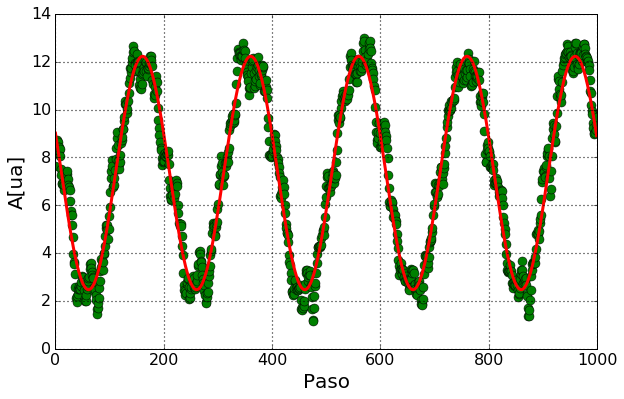
\includegraphics[width=0.8\textwidth]{fig/polarimetro/polarizacion_laser}
        \caption{Antes de la fibra óptica}
        \label{fig:polarimetro/polarizacion_laser}
    \end{subfigure}
    \begin{subfigure}[b]{0.5\textwidth}
        \centering
        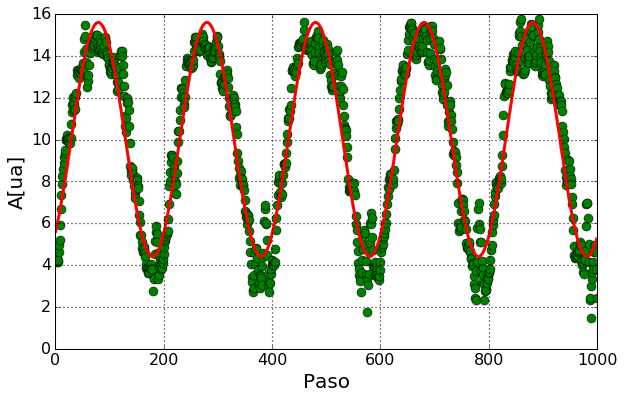
\includegraphics[width=0.8\textwidth]{fig/polarimetro/polarizacion_fibra}
        \caption{Después de la fibra óptica}
        \label{fig:polarimetro/polarizacion_fibra}
    \end{subfigure}
    \caption{Mediciones del polarimetro antes y después de la fibra óptica del SPIM para el láser azul}
\end{figure}

Al no poder controlar la intensidad del haz a la entrada de la fibra se debió intercalar filtros neutros en el camino del haz y amplificar la señal del fotodiodo. Esto conlleva a la presencia de ruido en la señal del fotodiodo, que es amplificada. 

La disposición de filtros neutros se mantuvo constante en todas las mediciones, así no se generaba diferencias de potencias que generen diferencias en el coeficiente $\alpha$. 

Al poder efectuar el ajuste correctamente en el conjunto de datos, en este caso de 4000 puntos, se puede descartar que la polarización cambie el intervalos de tiempo menores a 2s. Este ajuste a su vez descarta la polarización aleatoria, por lo que permitiría al SPIM hacer análisis de anisotropía (intercalando en el riel a la salida del colimador láminas retardadoras).

Para completar el análisis, se calculan los coeficientes $\alpha$, con la formula \ref{eq:polarizacion/alpha}. Si al atravezar la fibra se mantiene el coeficiente se mantiene, la fibra no altera la polarización a menos de una rotación de los ejes. Estos coeficientes se calculan a partir de el ajuste efectuado. 

Antes de la fibra el coeficiente obtiene un valor $\alpha = (0,664\pm 0,025)$ y después de la fibra $\alpha = (0,660\pm0,029)$. Esto determina que la fibra mantiene, dentro del error, la polarización para el laser azul, que es eliptica.

Se hicieron las mismas mediciones para los otros láseres del setup, uno verde ($\lambda = 532$nm) modelo Coherent 315M-100 y uno rojo HeNe Melles Griot 25-LHP-151-230 (ya usado previamente), y estas mediciones está condensadas en la tabla \ref{tbl:polarimetro/mediciones}

\begin{table}[H]
    \centering
    \begin{tabular}{c|c|c}
        Laser  & $\alpha_{\text{laser}}$ & $\alpha_{\text{fibra}}$ \\ \hline
        Azul   & 0,664$\pm$0,025   & 0,660$\pm$0,029   \\
        Verde  & 0,571$\pm$0.086   & 0.539$\pm$0,064   \\
        Rojo   & 0,8916$\pm$0,0027 & 0,3482$\pm$0,0014 \\
    \end{tabular}
    \caption{Mediciones del polarimetro en el setup del SPIM para diferentes haces, antes y después de la fibra óptica}
    \label{tbl:polarimetro/mediciones}
\end{table}

Se observa que para el láser verde y azul la polarización se mantiene, dentro del error, pero no es el caso para el láser rojo. No es posible descartar un error propio de la lámina polarizadora, por lo que sería conveniente recurrir a un polarizador más cercano al ideal y repetir estas mediciones.


    \section{Conclusiones}
        Respecto al perfilador, con el prototipo final se logró mediciones con el mismo error cometido, un 5\%, que el sistema manual, además se observó correlación entre las mediciones. 

        La velocidad de adquisición, determinada por la velocidad del motor y la velocidad de transferencia de datos, permite observar el perfil en tiempo real, es decir unas 24 veces por segundo. De esta forma es posible alinear y observar cambios del tamaño del haz al mismo tiempo, mejorando el proceso.

        Además de mejorar la velocidad de adquisición de un perfil de haz, este instrumental permite medir sin desarmar el setup del SPIM, lo que permitiría ser utilizado fácilmente en cualquier experiencia del laboratorio y eventualmente adaptarlo para otras aplicaciones.

        La tecnología desarrollada para el perfilador permitió rápidamente readaptarla para la creación de un polarímetro, también portátil, con el objetivo de observar la polarización del haz en el microscopio SPIM.
        
        Dado el material polarizante a usar, se pasó a calibrarlo. Esta calibración determinó que una lámina del material distan de ser un polarizador perfecto, al tener transferencia en el eje perpendicular al eje principal. Sin embargo, no es necesario para descartar cambios en la polarización en el tiempo o polarización aleatoria. Estas láminas no permiten diferenciar un haz linealmente polarizado a uno elipticamente polarizado. 

        Con las láminas calibradas se hicieron mediciones de la polaización antes y después de la fibra del SPIM, para varios laseres. Se observó que la polarización no cambió en los 2s de medición, lo que es un fuerte indicador de la constancia de dicha. Además la polarización de los laseres azul y verde se mantuvo al atravezar la fibra, pero no se observó el mismo resultado para el laser rojo. Es conveniente repetir estas mediciones con un polarizador más cercano al ideal.
    %\section{Agradecimientos}
    %\begin{itemize}
    %    \item A mi director Hernan Grecco
    %    \item Juan Bujjamer
    %    \item Bruno Moretti
    %    \item A la comunidad del LEC
    %    \item Martin Labate, por ayudarme a imprimir las piezas
    %\end{itemize}

    \begin{thebibliography}{3}
        \bibitem{huisken2004}
        J. Huisken, J. Swoger, F. Del Bene, J. Wittbrodt, E. H. K. Stelzer, ''Optical Sectioning Deep Inside Live Embryos by Selective Plane Illumination Microscopy'', \emph{Science} 13 August 2004, Vol. 305 no. 5686 pp. 1007-1009.
        \bibitem{svelto}
            O. Svelto, Principles of Lasers, 2010, Springer-Verlag
        \bibitem{goldstein_collett}
            D. Goldstein and E. Collett, Polarized Light, 2nd ed., CRC Press (2003)
        \bibitem{thorlabs_profiler} 
            Dual Scanning Slit Beam Profiler, {\footnotesize \url{https://www.thorlabs.com/thorproduct.cfm?partnumber=BP209-VIS}}
        \bibitem{soma}
            Proyecto SOMA, \url{http://lec.df.uba.ar/soma}
        \bibitem{thorlabs_cage}
            Cage Systems Ø1'', \url{https://www.thorlabs.com/navigation.cfm?guide_id=2002}
       \bibitem{42BYGHW609}
            42BYGHW609 Stepper Motor, \url{https://goo.gl/AbBvMW}
        \bibitem{8H2A28402}
            Nema 8, 8H2A, Miniature Stepper Motors -20mm(1.8 degree), \url{http://goo.gl/qSGui9}
        \bibitem{arduino}
            Arduino Development Platform, \url{http://www.arduino.cc}
        \bibitem{teensy}
            Teensy Development Board,  \url{https://www.pjrc.com/teensy/teensy31.html}
        \bibitem{particle_photon}
            Particle Photon Development Board, \url{https://docs.particle.io/guide/getting-started/intro/photon/}
        \bibitem{pololu}
            Pololu A4988 Stepper Motor Driver Carrier,  \url{https://www.pololu.com/product/1182}
        \bibitem{fds010} 
         Thorlabs FDS010 photodiode \url{https://www.thorlabs.com/thorcat/0600/FDS010-SpecSheet.pdf}
        \bibitem{thorlabs_fc}
            Fixed Focus Collimation Packages: FC/PC Connectors, \\ \url{https://www.thorlabs.com/newgrouppage9.cfm?objectgroup_id=944}
    \end{thebibliography}

    \clearpage
    \appendix
    \section{Diseños mecánicos del perfilador}
    \subsection{Tambor del perfilador}
    \vfill
    \begin{figure}[H]
    \centering
    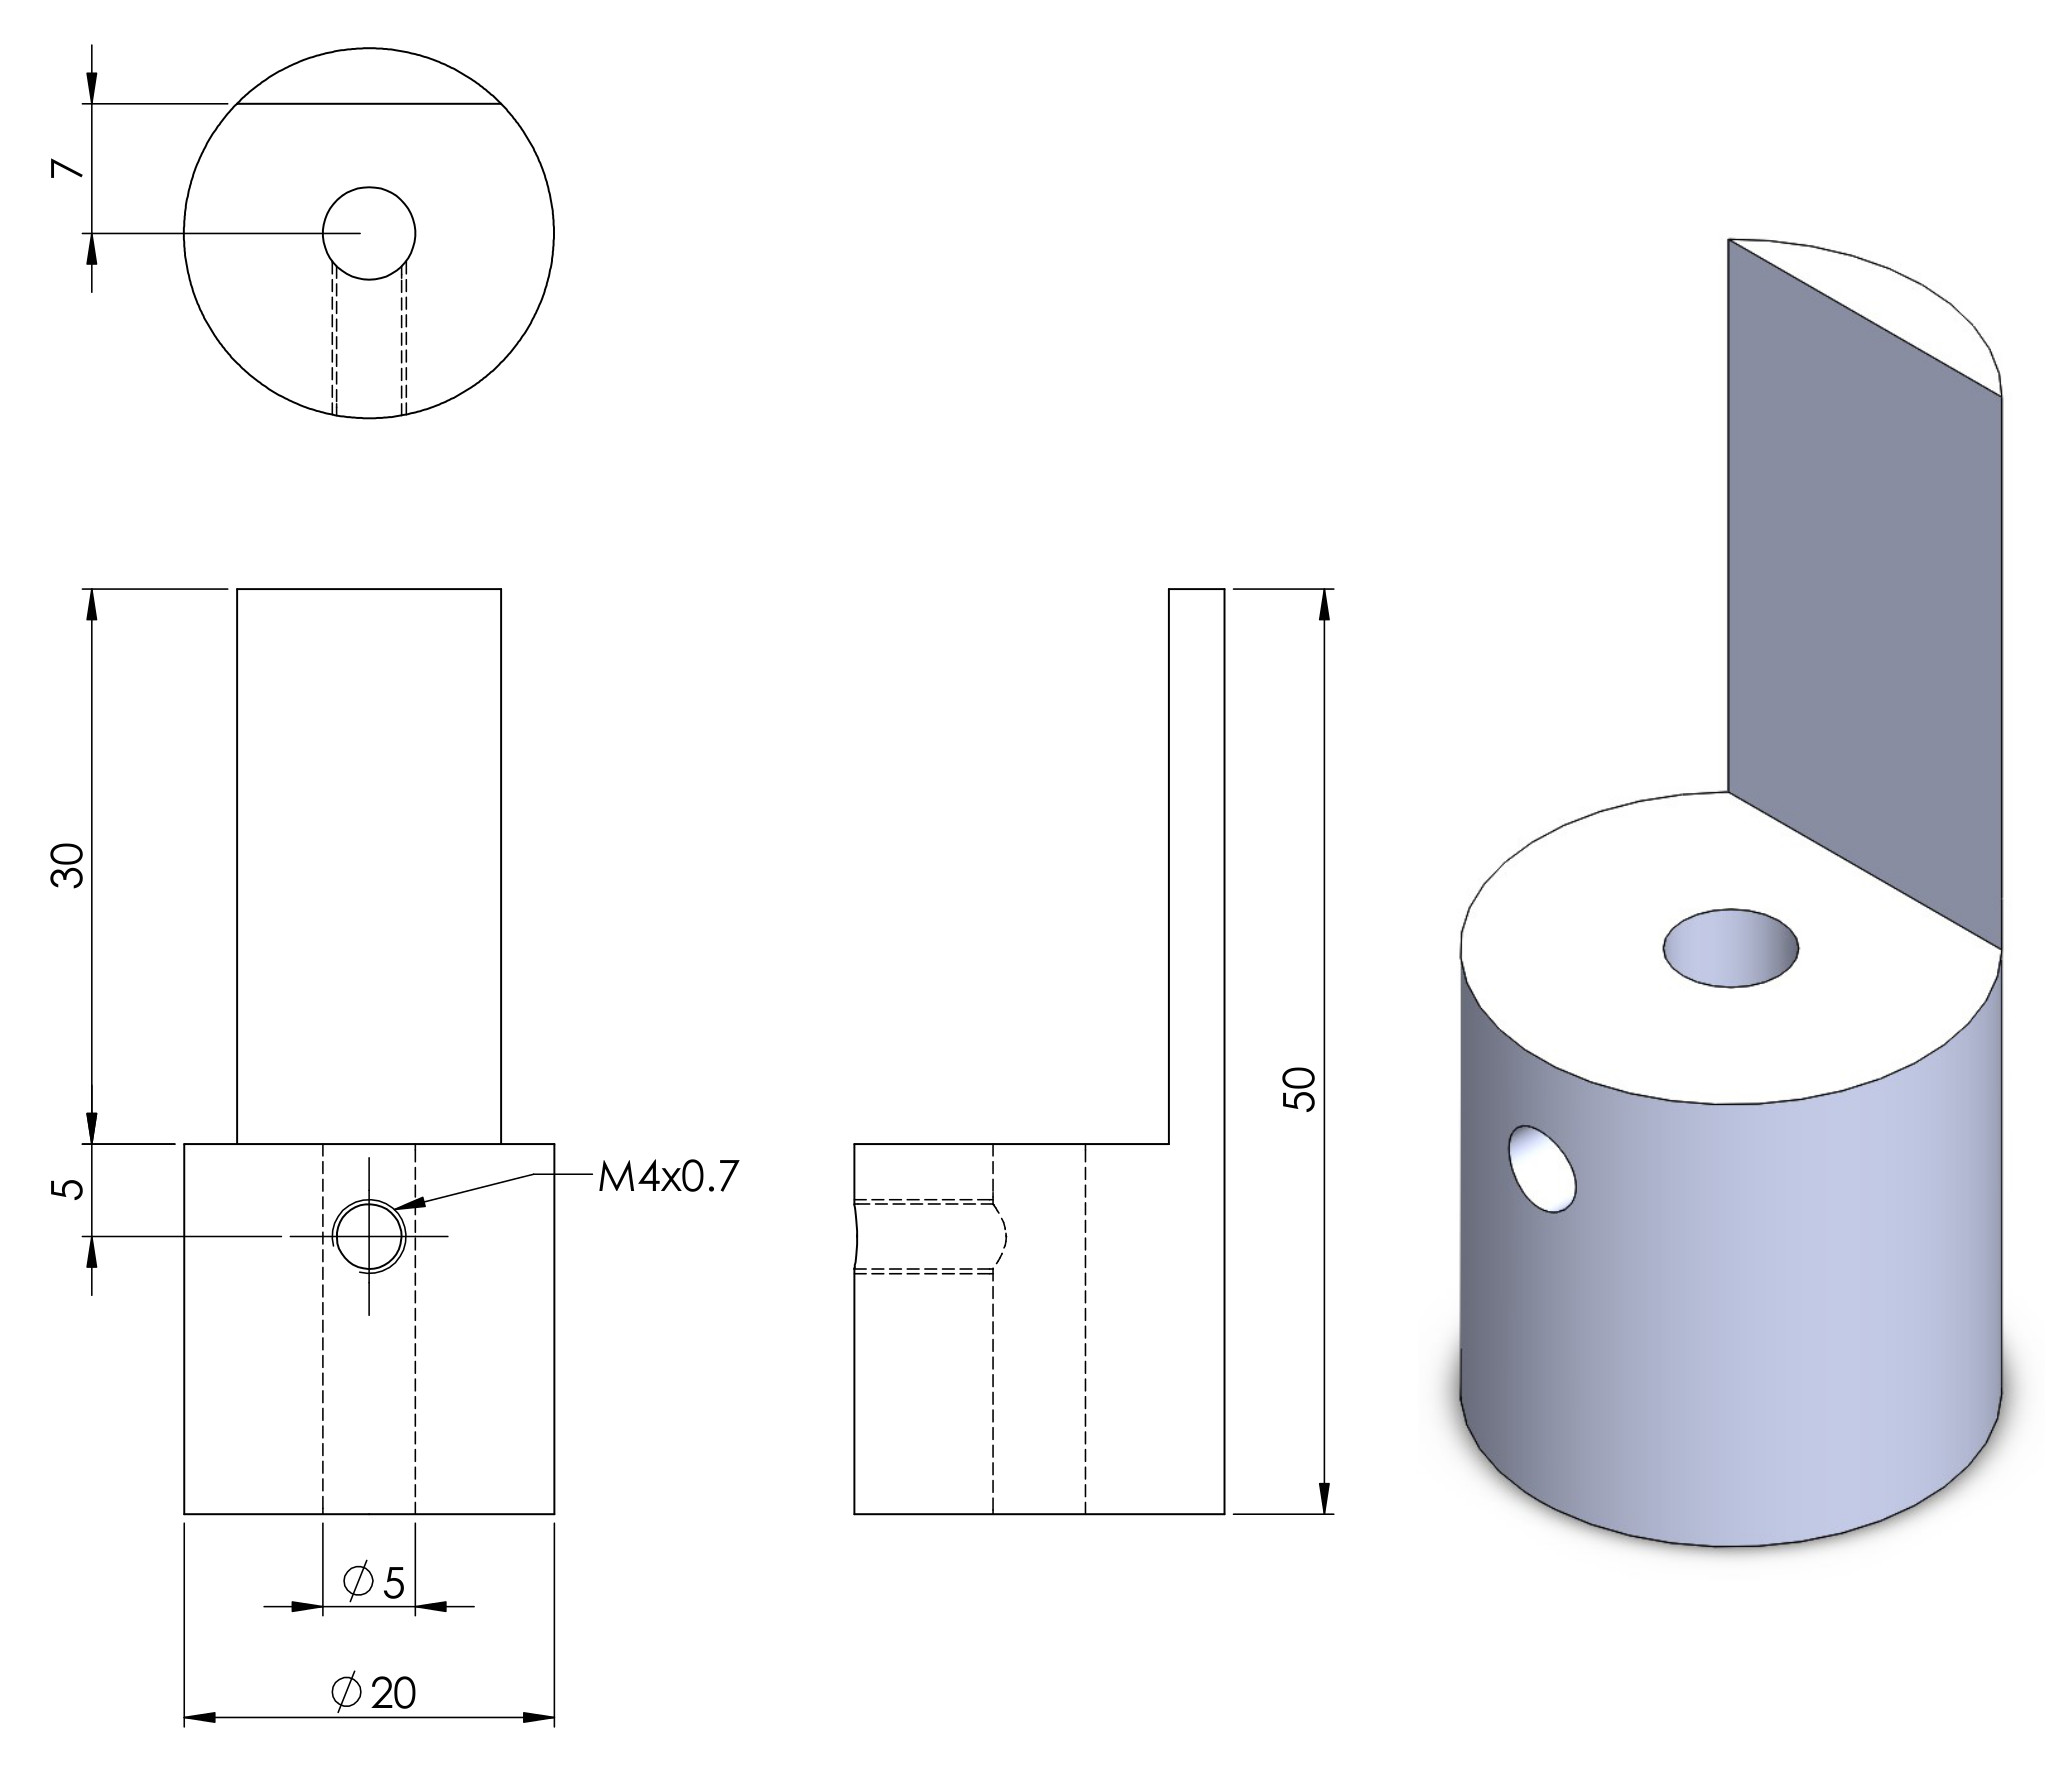
\includegraphics[width=0.8\textwidth]{fig/perfilador/tambor_mecanico}
    \caption{Dibujo mecánico del tambor. No está a escala}
    \label{fig:perfilador/tambor_plano}
    \end{figure}
    \vfill

    \clearpage
    \subsection{Soporte}
    \vfill
    \begin{figure}[H]
    \centering
    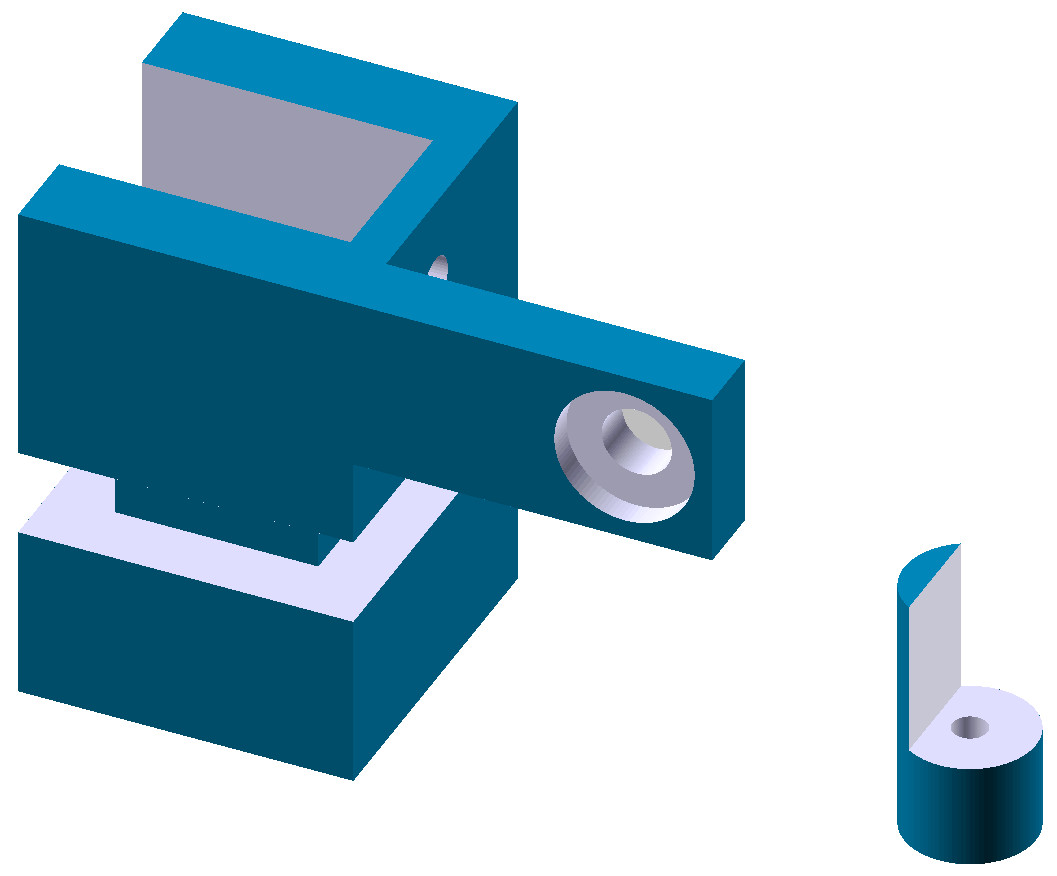
\includegraphics[width=0.8\textwidth]{fig/perfilador/soporte_v4_mecanico}
    \caption{Dibujo mecánico del soporte del perfilador. No está a escala}
    \label{fig:perfilador/soporte_plano}
    \end{figure}
    \vfill

    \clearpage
    \section{Diseños mecánicos del polarimetro}
    \subsection{Soporte}
    \begin{figure}[H]
    \centering
    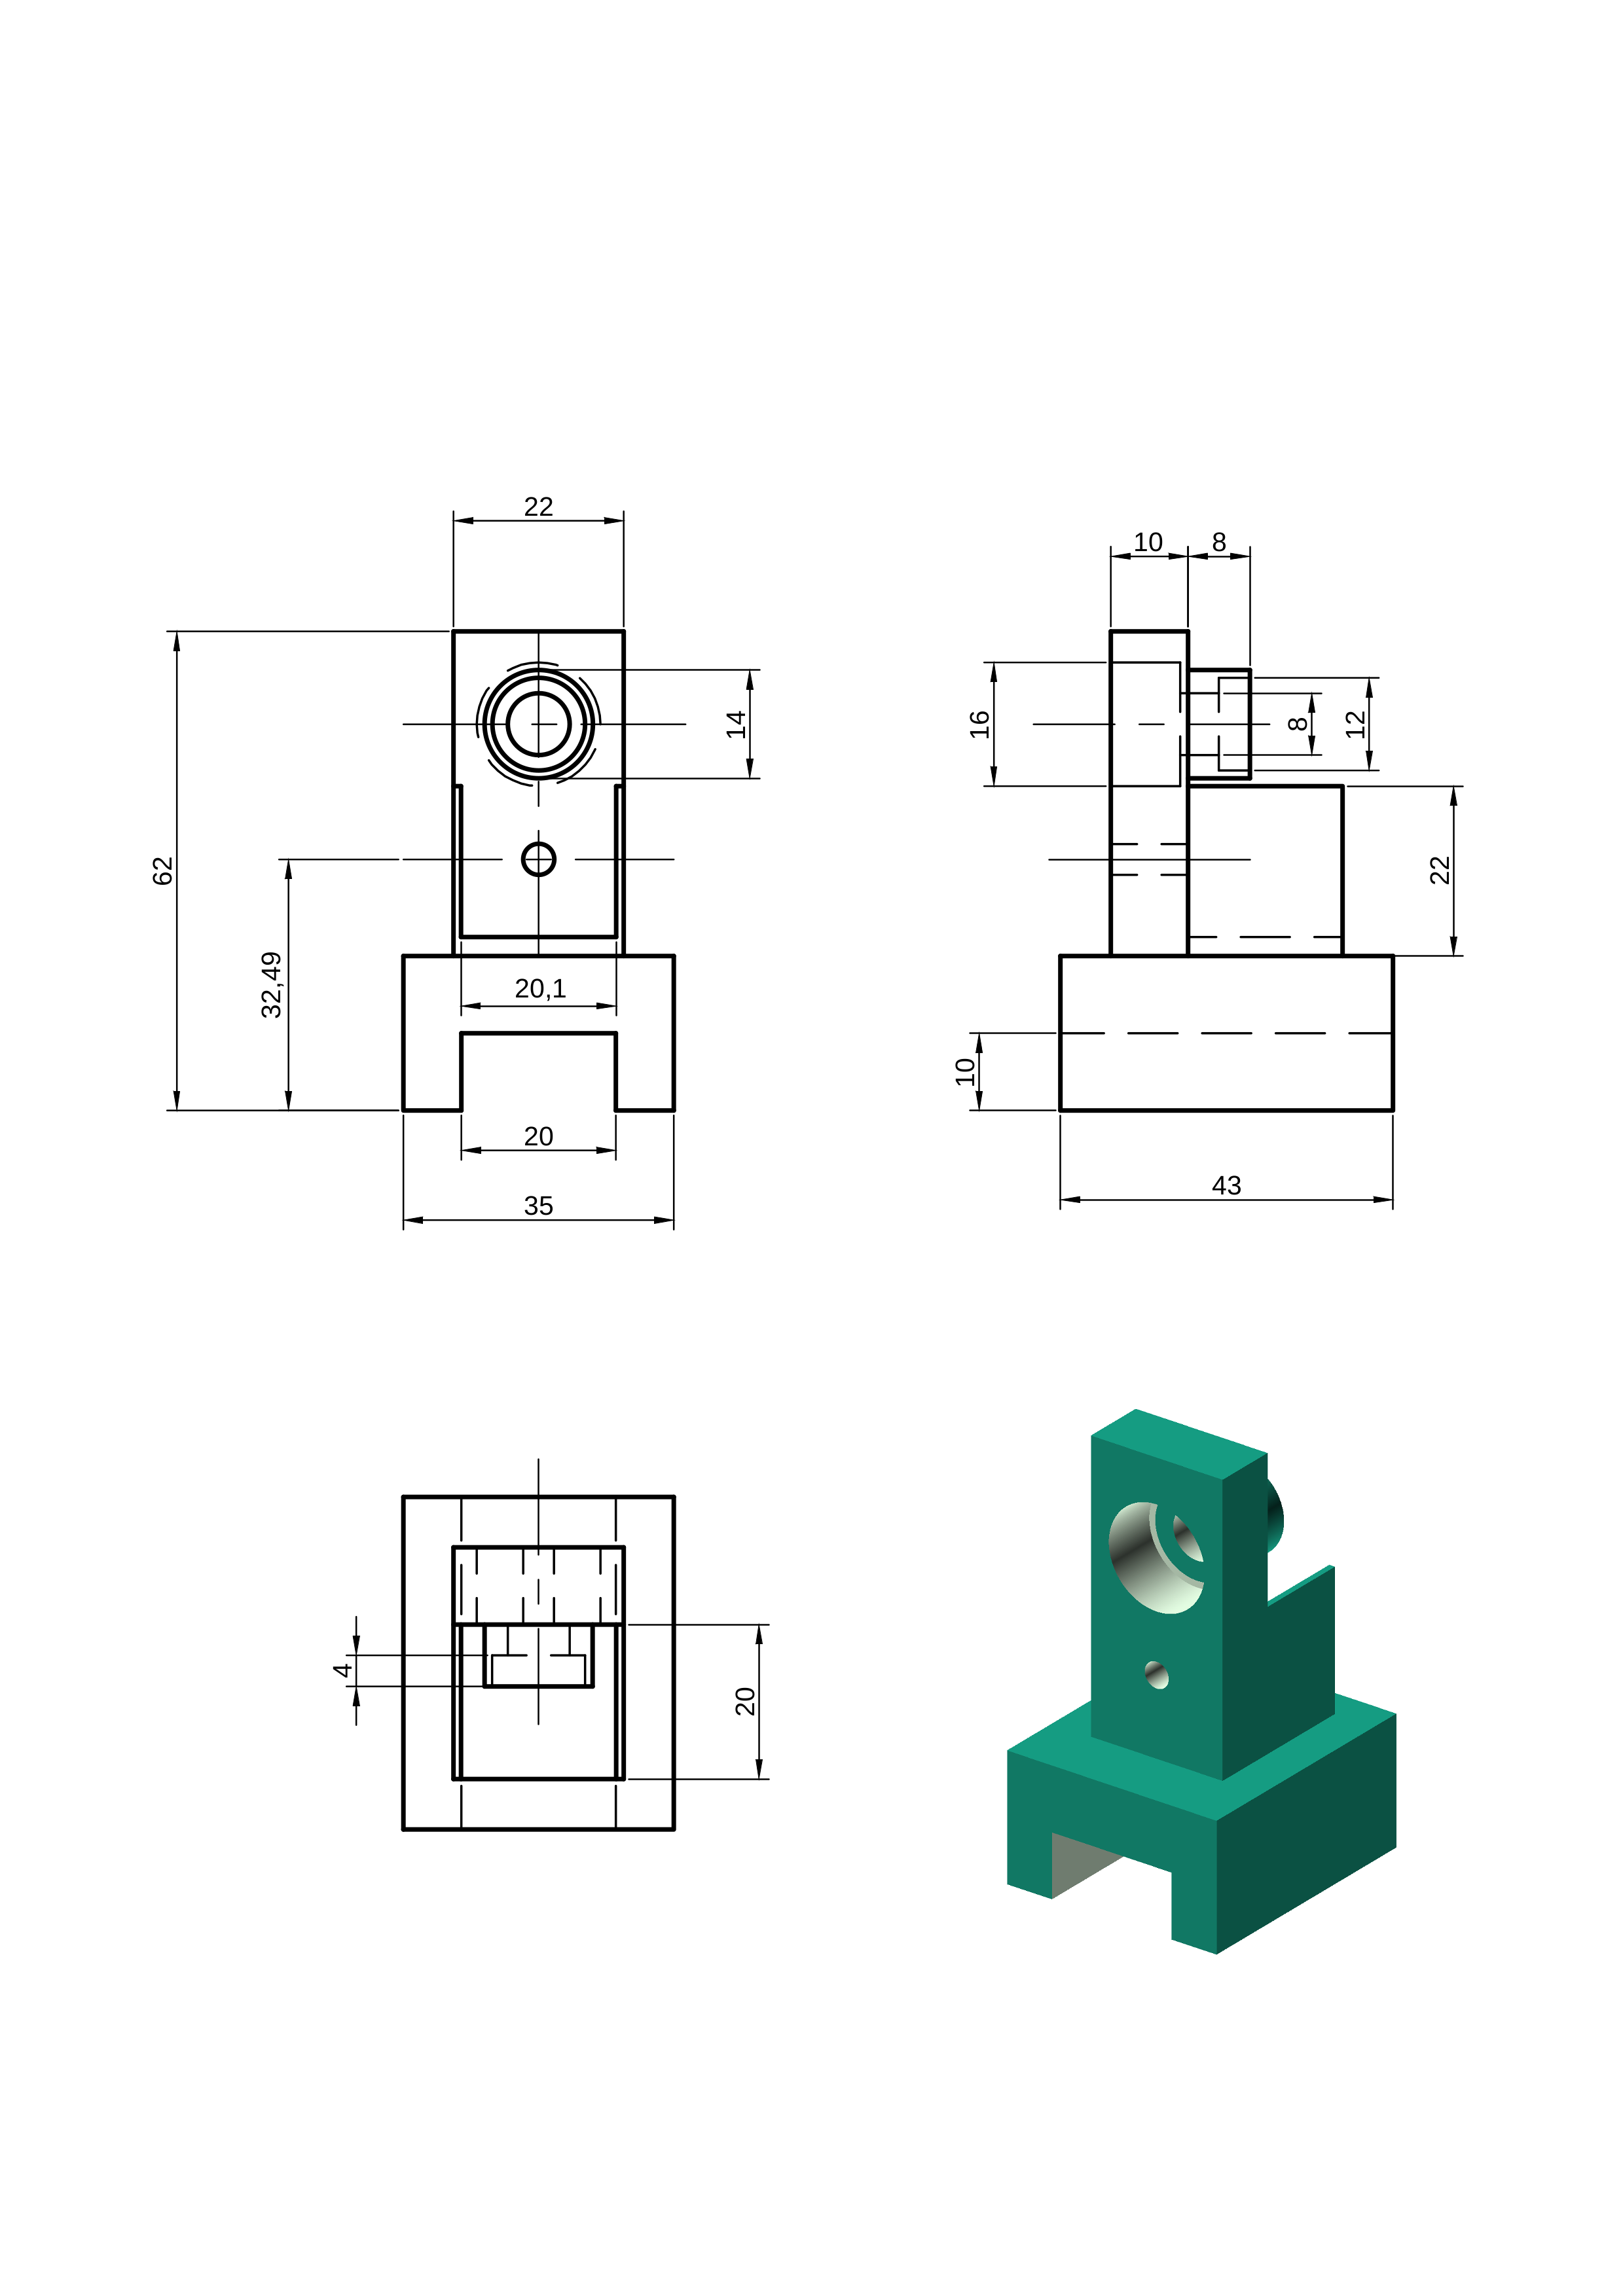
\includegraphics[width=0.8\textwidth]{fig/polarimetro/soporte_mecanico}
    \caption{Dibujo mecánico del soporte del polarimetro. No está a escala}
    \label{fig:polarimetro/soporte_plano}
    \end{figure}
    \vfill

    \subsection{Engranajes}
    \vfill
    \begin{figure}[H]
    \centering
    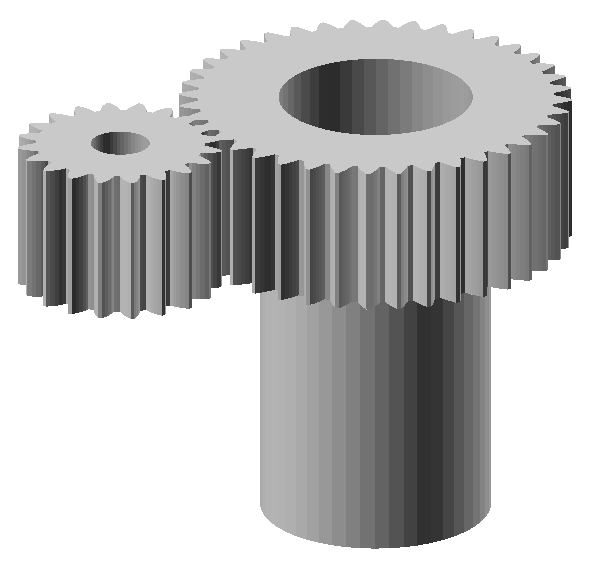
\includegraphics[width=0.8\textwidth]{fig/polarimetro/engranajes_mecanico}
    \caption{Dibujo mecánico de los engranajes. No está a escala}
    \label{fig:polarimetro/engranajes_plano}
    \end{figure}
    \vfill


    \clearpage
    \section{Diseños de la electrónica}
    \vfill
    \begin{figure}[H]
    \centering
    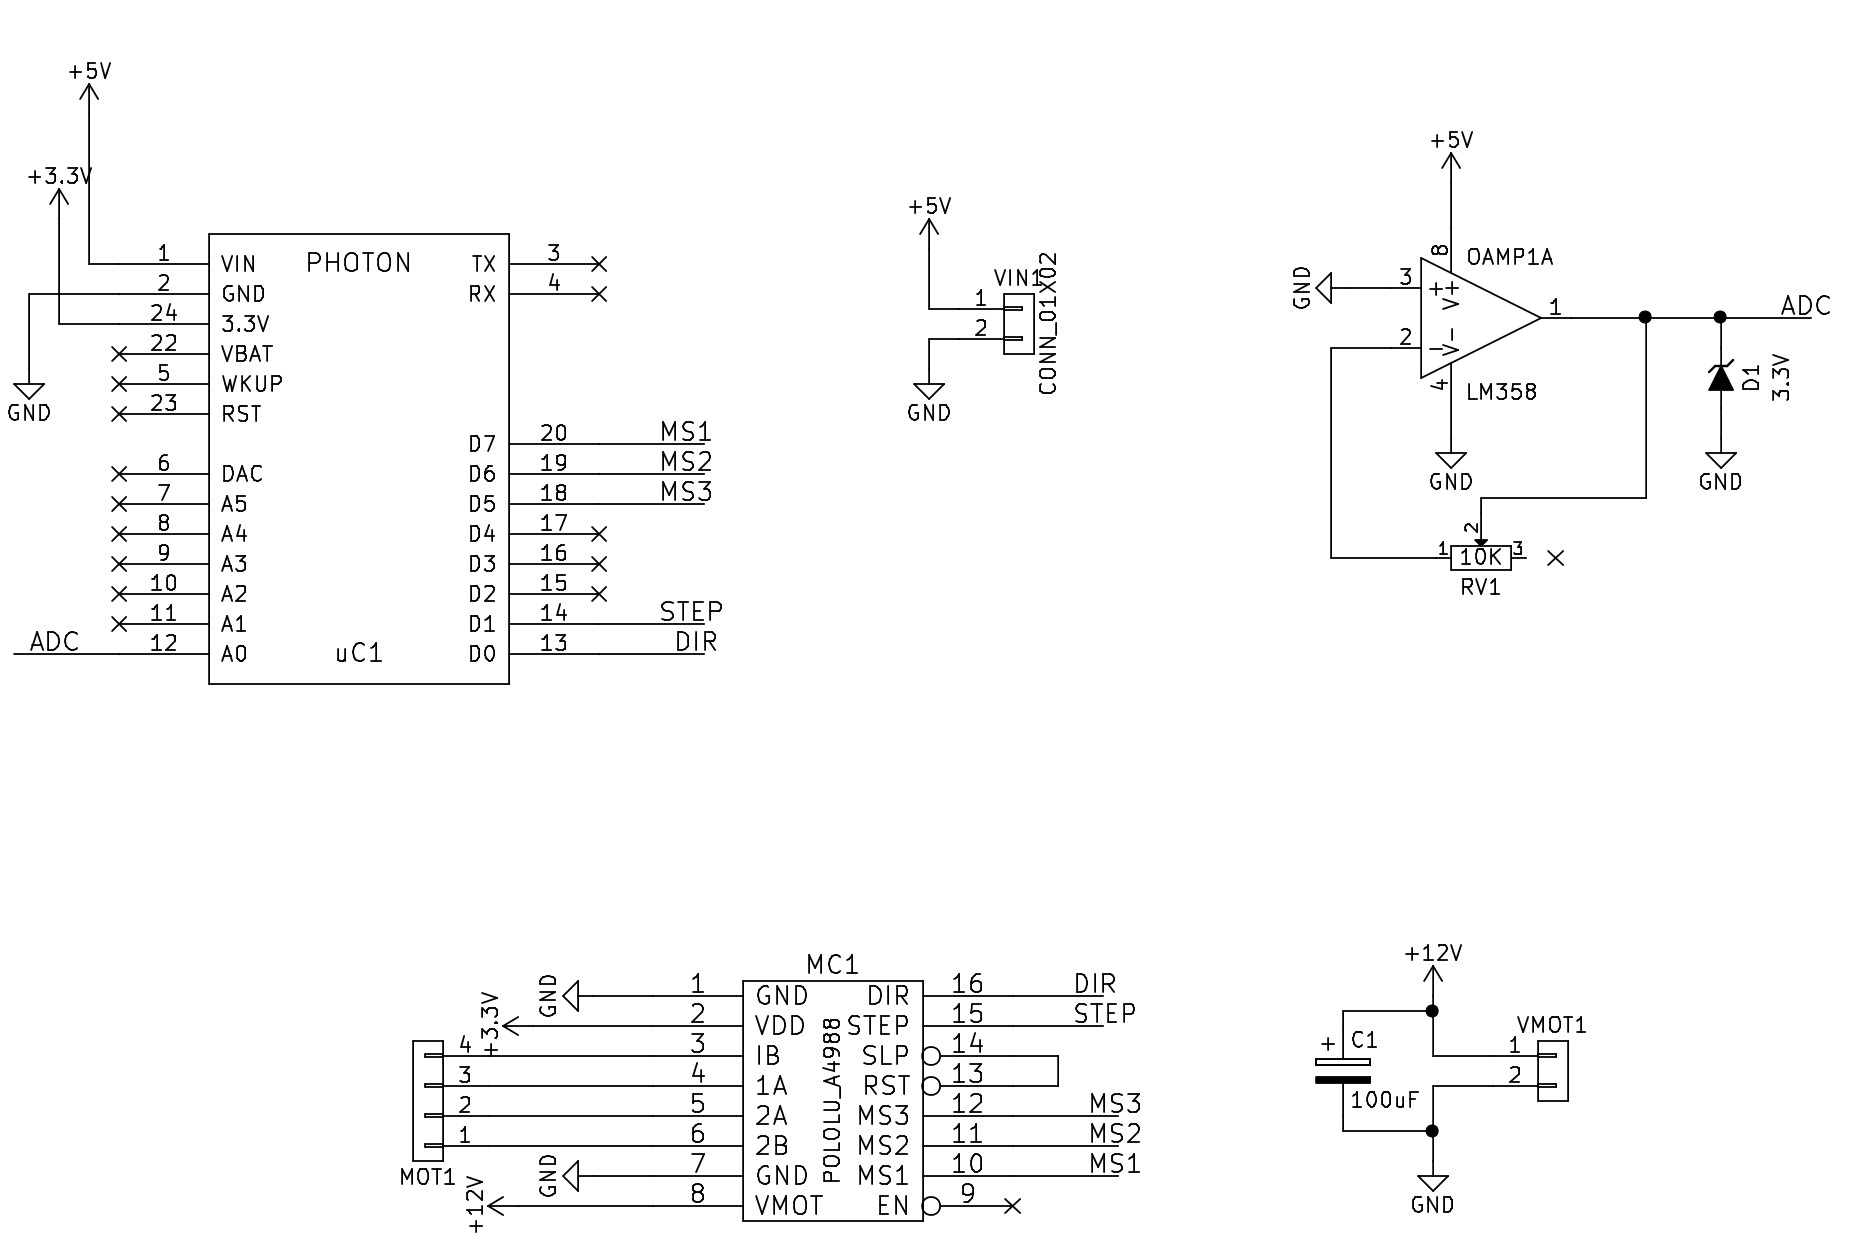
\includegraphics[width=15cm]{fig/circuito/circuito_esquematico}
    \caption{Esquematico del circuito eléctronico de adquisición.}
    \label{fig:circuito/esquematico}
    \end{figure}
    \vfill
    \begin{figure}[H]
    \centering
    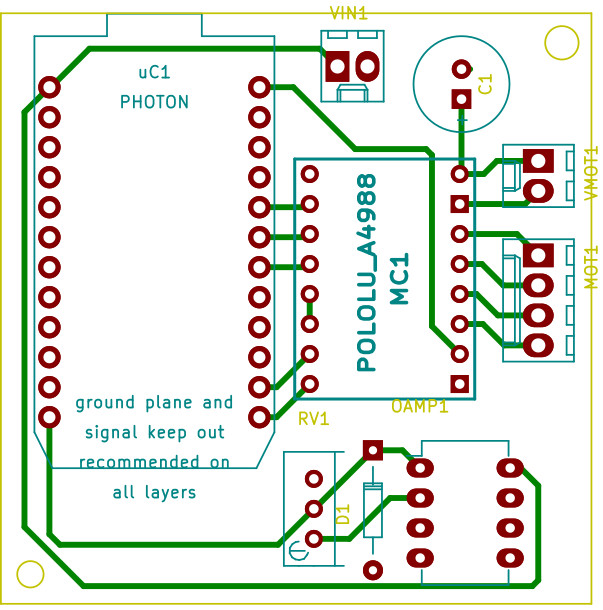
\includegraphics[width=10cm]{fig/circuito/circuito_pcb}
    \caption{Circuito impreso de adquisición. Escala 2:1}
    \label{fig:circuito/pcb}
    \end{figure}
    \vfill
\end{document}
